
% to choose your degree
% please un-comment just one of the following
\documentclass[bsc,frontabs,twoside,singlespacing,parskip,deptreport]{infthesis}     % for BSc, BEng etc.
% \documentclass[minf,frontabs,twoside,singlespacing,parskip,deptreport]{infthesis}  % for MInf
%\usepackage{subcaption}
\usepackage{graphicx}
%\usepackage{caption}
\usepackage{subfigure}

% For citations
\usepackage{natbib}
\usepackage[utf8]{inputenc}
\usepackage{fourier} 
\usepackage{array}
\usepackage{makecell}

% For algorithms
\usepackage{algorithm}
\usepackage{algorithmic}

\usepackage{listings}
\usepackage{xcolor}
\lstset { %
    language=C++,
    backgroundcolor=\color{black!5}, % set backgroundcolor
    basicstyle=\footnotesize,% basic font setting
}

\usepackage{enumerate}

\graphicspath{ {./images/} }
\bibliographystyle{plain}


\usepackage[hyphens]{url}
\urlstyle{same}
\usepackage{hyperref}

\usepackage{amsmath}

\DeclareMathOperator{\atan}{atan2}
\DeclareMathOperator{\acos}{acos}

\newcommand{\threat}{malicious \hspace{}}
\newcommand{\Threat}{Malicious \hspace{}}
\newcommand{\nonthreat}{benign \hspace{}}
\newcommand{\Nonthreat}{Benign \hspace{}}

\newcommand{\E}[2]{\mathbb{E}\left[{#1} | #2 \right]}
\newcommand{\usvset}{\mathrm{U}}
\newcommand{\intruderset}{\mathrm{B}}
\newcommand{\threatintruderset}{\mathrm{I}}
\newcommand{\threatintruder}{\mathcal{\iota}}
\newcommand{\observationset}{\mathcal{O}}
\newcommand{\agentassignment}[1]{\mathrm{H}_{#1}}
\newcommand{\swarmassignment}[1]{\mathcal{A}_{#1}}
\newcommand{\agentmotiongoal}[1]{\mathrm{M}_{#1}(\mathcal{O}, \mathcal{A})}
\newcommand{\agentlocation}[1]{\mathrm{l_{#1}}}
\newcommand{\agentcommand}[1]{\phi_{#1}}%{(\agentmotiongoal{#1}})}
\newcommand{\agent}[1]{a_{#1}}
\newcommand{\usvagent}[1]{u_{#1}}
\newcommand{\intruderagent}[1]{b_{#1}}
\newcommand{\agentheading}{\theta}
\newcommand{\agentspeed}{s}
\newcommand{\deltaspeed}{\Delta~\agentspeed}
\newcommand{\deltaheading}{\Delta~\agentheading}
\newcommand{\maxsym}{max}
\newcommand{\maxdeltaspeed}{\deltaspeed^{\maxsym}}
\newcommand{\maxdeltaheading}{\deltaheading^{\maxsym}}
\newcommand{\maxagentspeed}{\agentspeed^{\maxsym}}
\newcommand{\aggression}{\alpha}
\newcommand{\pthreat}{p_{threat}}
\newcommand{\threatprob}[1]{P(\intruderagent{#1} \in \threatintruderset|\observationset)}
\newcommand{\taskallocation}[1]{\mathrm{H}_{#1}}
\newcommand{\usvtaskallocation}{\taskallocation{\usvagent{j}}}
\newcommand{\totaltaskset}{\agentassignment{g} \cup \agentassignment{o} \cup \agentassignment{d}}


\renewcommand\theadalign{bc}
\renewcommand\theadfont{\bfseries}
\renewcommand\theadgape{\Gape[4pt]}
\renewcommand\cellgape{\Gape[4pt]}



\begin{document}

\title{Threat Detection and Reaction System using a team of Unmanned Sea Vessels (USVs) }

\author{Dylan Angus}

% to choose your course
% please un-comment just one of the following
%\course{Artificial Intelligence and Mathematics}

% to choose your report type
% please un-comment just one of the following
%\project{Undergraduate Dissertation} % CS&E, E&SE, AI&L
%\project{Undergraduate Thesis} % AI%Psy

% The document structure should include:
% \begin{itemize}
% \item
% The title page  in the format used above.
% \item
% An optional acknowledgements page.
% \item
% The table of contents.
% \item
% The report text divided into chapters as appropriate.
% \item
% The bibliography.
% \end{itemize}

% Commands for generating the title page appear in the skeleton file and
% are self explanatory.
% The file also includes commands to choose your report type (project
% report, thesis or dissertation) and degree.
% These will be placed in the appropriate place in the title page. 

% The default behaviour of the documentclass is to produce documents typeset in
% 12 point.  Regardless of the formatting system you use, 
% it is recommended that you submit your thesis printed (or copied) 
% double sided.

% The report should be printed single-spaced.
% It should be 30 to 60 pages long, and preferably no shorter than 20 pages.
% Appendices are in addition to this and you should place detail
% here which may be too much or not strictly necessary when reading the relevant section.


% Divide your chapters into sub-parts as appropriate.


% Note that citations 
% (like \cite{P1} or \cite{P2})
% can be generated using {\tt BibTeX} or by using the
% {\tt thebibliography} environment. This makes sure that the
% table of contents includes an entry for the bibliography.
% Of course you may use any other method as well.


% There are various documentclass options, see the documentation.  Here we are
% using an option ({\tt bsc} or {\tt minf}) to choose the degree type, plus:
% \begin{itemize}
% \item {\tt frontabs} (recommended) to put the abstract on the front page;
% \item {\tt twoside} (recommended) to format for two-sided printing, with
%   each chapter starting on a right-hand page;
% \item {\tt singlespacing} (required) for single-spaced formating; and
% \item {\tt parskip} (a matter of taste) which alters the paragraph formatting so that
% paragraphs are separated by a vertical space, and there is no
% indentation at the start of each paragraph.
% \end{itemize}


\project{4th Year Project Report}

\date{\today}

\abstract{
In this report, we detail how we tackled two difficult tasks. Identifying potential threats in a densely populated trade route and coordinating a team of USV's to manoeuvre through this route, avoiding collisions with themselves and other vessels, while  making distributed decisions concurrently, for the purpose of investigating and handling potential threats. We demonstrate how we introduce a novel threat detection system using real-world vessel traffic data. Then, we describe how we have implemented a state of the art threat reaction system for a team of Unmanned Sea Vessels (USVs) using \texttt{C++} and \texttt{ROS}, allowing for hardware extraction and potential extension to actual Autonomous Sea Vessels. Furthermore, we then describe how the generalisation of the threat detection system affects how well the reaction system can delay the threats from reaching the asset. \inlinecomment{Discuss Results}


% This is an example of {\tt infthesis} style.
% The file {\tt skeleton.tex} generates this document and can be 
% used to get a ``skeleton'' for your thesis.
% The abstract should summarise your report and fit in the space on the

% first page.
%
% You may, of course, use any other software to write your report,
% as long as you follow the same style. That means: producing a title
% page as given here, and including a table of contents and bibliography.
}

\maketitle

% \section*{Acknowledgements}
% I would like to acknowledge 

\tableofcontents

%\pagenumbering{arabic}


\chapter{Introduction}
\section{Motivation}
Countries around the world have been investing resources in Unmanned Sea Vessels (USVs) that can operate autonomously in a marine environment \cite{usvcase}.  Investing in this technology is important because they can save countries/companies not just money but also lives. Marine assets like oil tankers, cargo-ships and aircraft carriers are at risk due to being fairly non-manoeuvrable while carrying important cargo. This was unfortunately proven to be true on 12 October 2000, when the USS Cole guided-missile destroyer was the target of a terrorist attack while it was being refuelled \cite{combs2009encyclopedia}. The attack was caused by a small fiberglass boat carrying C4 explosives approaching the destroyer and blowing a hole in the ships hull. Something that could have been avoided using the system described in this report. Firstly, the threat detection system would alert them of a potential threat, allowing them to take defensive manoeuvres, like calling for back-up. Then  the team of USV's could have been used to delay the threats for as long as possible, lending time for back-up to reach or for them to escape, without risking any human lives.

\section{Context}
Some developed countries have managed to develop systems that can perform various tasks patrolling a specified area, observing suspicious vessels and delaying intruders from an important asset. Performing these tasks alone is a difficult feat and present their own challenges \cite{usvcase}\cite{wolf2017caracas}\cite{raboin2013model}. However, juggling these tasks in tangent while manoeuvring through a popular vessel route is a non-trivial task in itself. Though work has been put into deriving how to delay intruding vessels that may come close to an asset that's it's in charge of protecting \cite{raboin2013model} while avoiding obstacles \cite{gupta2015block}\cite{marzoughi2018collision}. It should only do this when it is absolutely sure that it poses a threat. Hence, there is a need for a robust threat detection system that realistically models vessel traffic behaviour. It should be noted that understanding maritime traffic patterns and modelling normal vessel behaviour on a trade route is an invested in and active area of research. This has been facilitated by the build-up of terrestrial networks and constellations of Automatic Identification System (AIS) receivers. Which allow for ship movement information in both coastal and open waters becoming available \cite{perez2009automatic}. Furthermore, AIS data has been analysed and used to perform various tasks such as route detection, anomaly detection and motion prediction\cite{pallotta2013vessel} \cite{ristic2008statistical} \cite{kowalska2012maritime}. Thus, it is reasonable to believe that a USV squad would have access to this historical data to model normal vessel movement for motion prediction and threat detection. However, to our knowledge no one has incorporated and evaluated the two systems together.


\section{Problem Statement}
The problem this project seeks to solve is that of detecting, investigating and then reacting to malicious vessels pretending to be benign ships. This problem further breaks down into the following sub-problems discussed in the sections below:

\subsection{Modelling Vessel Traffic}
A model defining normal vessel behaviour is needed by both the threat detection and reaction systems. Additionally, this model must reflect the types of behaviours observed in the real-world. Finally, the model must be capable of being sampled from for numerous intruders simultaneously, at a high enough frequency for the systems to operate optimally. 
\subsection{Threat Detection}
This is the problem of identifying abnormal behaviour from malicious boats posing as benign vessels. Furthermore, because we don't want the threat reaction system disturbing benign vessels, and failure to alert the threat reaction system could result in expensive damage in property and possibly loss of human lives. Thus, this system must be as accurate and as quickly as possible. 

\subsection{Threat Reaction}
This is the problem of controlling a distributed team of USV's concurrently in continuous space to react to potential threats. This problem can actually be modelled as the highly researched Multi-Robot Task Allocation problem. In our project these are the tasks the USVs have to balance between:

\begin{itemize}
    \item Observing vessels that could be potential threats
    \item Maintaining advantageous positioning of USVs around the asset
    \item Delaying any intruders classified as threats from reach the asset for as long as possible
\end{itemize}
Furthermore, the USVs must figure out away to balance between these tasks while not disturbing \nonthreatening vessels in the trade route and avoiding collisions.

\section{Challenges}
As addressed in \cite{raboin2013model} the high-level task planning and behaviour optimisation for a team of USVs guarding an asset is an instance of the MT-MR-TA (multi-task robots, multi-robot tasks, time extended allocation) variant of task allocation problems. I address this by using the market-based exchange strategy proposed in \cite{raboin2013model}. In which a local search is performed in the space of USV task assignments and assignments are evaluated using a model-predictive simulation. Each task will be executed like a corresponding parameterized behaviour like in \cite{raboin2013model}.
Unfortunately, there was not an open-source implementation of this system. Hence, we had to spend a lot of time implementing the threat reaction system described in \citep{raboin2013model} from scratch. Though, we deviated from their implementation at certain points. These deviations are declared and explained in \ref{chap:reaction}.

\section{Project Structure}
In the following sections I will contrast and compare similar topics in literature similar to that of my project. Then in place of a typical "Methodology" I split it into three different sections. Each of those sections describe the problem thoroughly, then describe how we solve it. Following this I will describe the experiments I used to evaluate each sub-system. Lastly, I will discuss and evaluate the results from the experiments, summarise and conclude.

\chapter{Background}
\label{chap:background}
\section{Related Work}

\subsection{Multi-Agent Pursuit-Evasion Games}
The problem of guarding an asset using USV’s against other intruder vessels can be thought of a pursuit-evasion game where the evaders are trying to capture the asset which has been researched thoroughly. In the discrete case, agents are traversing on a graph where each agent occupies a single node on the graph and the edges are the reachable positions from a node. Pursuit-evasion games on graphs have been shown to have optimal policies to capture evaders with the minimum number of steps \cite{vieira2008optimal}. This could easily be adjusted suit our purposes by not allowing the pursuers to actually capture the evaders, but to just maximize the number of timesteps they can keep the evaders away from the asset. However, this does not generalize well to the real continuous world.

\subsection{Differential Games}
A closer approach to the problem addressed in this project is Issacs’ “Guarding a Territory” game \cite{isaacs1999differential}. In this game, a guard and an intruder start on separate parts of the map and the guard attempts to intercept an intruder as far as possible from the restricted territory while the intruder tries to get as close as possible to the territory. This game works on the continuous domain where the agents have constraints in the form of differential equations. For the single guard and intruder case with perfect information, an optimal solution can be found \cite{isaacs1999differential}. There have been several twists on this game investigated in the literature. In \cite{meng1999fuzzy} they introduced uncertainty over the agent’s and territory’s position. In \cite{raslan2016learning} the guard agents were taught an optimal policy to capture a superior intruder agent using Reinforcement Learning techniques.

\subsection{Multi-Agent Asset Protection}
\subsubsection{Interception Strategies}
In this section we discuss research that attempt to tackle the problem in a continuous space. A necessary and sufficient for the existence of decentralized motion control algorithm for a network if mobile robots to intercept an intruder on the boundary of a particular region was derived by \citet{marzoughi2018collision} and the algorithm proposed. 

\citet{gupta2015block} Investigated a set of different interception policies using a USVs as dynamic obstacles obstructing highly maneuverable threats from reaching a valuable naval asset. By applying a mirror transformation to the intruder's current state, \cite{gupta2015block} suggests a pursuit policy can be formed that always places the defending USV between the intruder and the asset. They also present a model-predictive method of calculating the motion goals for the defending USV and estimating the future intruder motions. Additionally, they showed how the predictive estimator is capable of generating a meta-model for the intruder's Behaviour and producing a probability distribution of the intruder's control actions based on a set of observable spatial features. 

\citet{moundegue2017fields} tackled the same problem as \cite{gupta2015block} but modelled it using the potential fields. Assuming the intruders have a positive attraction to the asset and a negative charge towards the USVs. Additionally, USVs had a limited field of vision to which to detect intruders and a limited range of communication between each other. The USVs also balanced between escorting the asset and blocking intruders. However, once an intruder was blocked it would go into a \emph{standby mode} and move away from the asset.

The paper most similar to problem addressed in this project is \citep{raboin2013model}. They developed a Behaviour-based control architecture to control a fleet of USVs to perform tasks such as guarding the asset, observing potential threats and delaying intruders once they are classified as threats. Their focus however, was on their model-predictive task allocation algorithm. This algorithm would forward project the state of USVs and intruders and evaluate which assignment of Behaviours performed the best. They found significant results with their algorithm vastly outperforming a heuristic task allocation baseline. 

However, they used a toy threat_classification detection system that would not generalize to the real world. Additionally, they made the assumption of knowing the correct model of the intruder which turns out to be very important as I will show later in this project.Thus, my contribution will be to integrating a threat_classification detection system that would generalize to the real world and evaluating how their system is capable of protecting an asset near a busy trade route and estimating the models of intruders that are classified as threats.

\subsection{Maritime Situational Awareness}
As mentioned in the introduction, a lot of work has been done in the field of maritime surveillance. This is because nations who fail to invest in this risk unauthorized maritime arrivals, prohibited imports/exports, maritime pollution, piracy, and maritime terrorism \cite{ristic2008statistical} such as the case of the missile destroyer \cite{combs2009encyclopedia}. Additionally, many papers attribute the increase in research into maritime surveillance because of the increase in self-reporting systems. Though these systems were first introduced mainly for the purpose of safety in navigation and collision avoidance they have since become an abundant and inexpensive source of information for maritime surveillance  \cite{kde}. The main self-reporting system Automatic Identification System (AIS) was made compulsory by the International Convention of Safety of life and sea (SOLAS) compulsory for most commercial ships (cargo, passenger, tankers, tugboats, etc.). AIS provides a means for ships to electronically broadcast ship data at regular intervals including vessel identification, position, course, speed and vessel type amongst other data. Thus, it was the spawn of numerous studies attempting to process and extract as much information as they could from AIS datasets. 

\subsubsection{Kernel Density Estimation (KDE)}
\label{sss:kde}
Kernel Density Estimation is a nonparametric probabilistic modelling technique which is normally used to approximate the distribution of a dataset $\mathcal{D}$. It does this by using so-called kernel functions $\kappa_h(\mathbf{x_i}, \mathbf{x_j})$, which estimate how similar $\mathbf{x_i} \text{and} \mathbf{x_j}$ are to each other. Where $h$, the bandwidth parameter, represents how sensitive your model will be to distance. Hence, at test time they model $P(\mathbf{x_*}|\mathcal{D}) = \sum_{x \in \mathcal{D}} \kappa_h(x_*, x)$

\cite{ristic2008statistical} used AIS data to extract motion patterns, using these patterns to construct motion anomaly detectors. They did this by using an \emph{adaptive kernel density estimator} (AKDE) to model normal vessel Behaviour by vessel class (if that information was available) and used that as the null hypothesis. Additionally, by using a particle filter with the weights for the particles given by the AKDE they were able to forward predict the motion of vessels based on their origin.

\begin{figure}
    \centering
    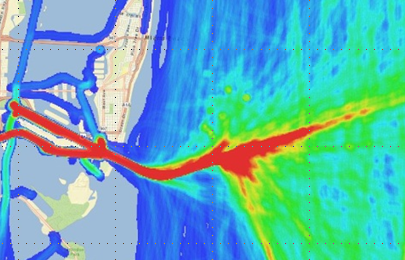
\includegraphics[]{report/images/ship_density_sm.png}
    \caption{KDE map of vessel traffic in a particular zone. Sourced from \href{https://marinecadastre.gov/ais/}{marine cadastre.}}
    \label{fig:density}
\end{figure}

\subsubsection{Gaussian Processes}
\label{sss:gp}
Gaussian Processes are bayesian non-parametric models which model distributions over functions $f$ with input $\mathbf{x}$. They assume that there is a probabilistic, zero-centred, Gaussian prior over all functions with input $\mathbf{x}$. Where, the covariance of the prior is calculated using a kernel function $\kappa(\mathbf{x_i}, \mathbf{x_j})$. Then use this to analytically construct a Gaussian distribution over the posterior distribution $P(f_* | y)$  with:

\begin{align}
E[f_*|\mathbf{y}] &= K(X_*, X)(K(X, X) + \sigma_y^2\mathbb{I})^{-1}\mathbf{y} \\
Cov[f_*|\mathbf{y}] &= K(X_*, X_*) - K(X_*, X)(K(X, X) + \sigma^2_y\mathbb{I})K(X, X_*)
\end{align}
where,

\hspace{0.5in} $K(X, Y)_{i, j} = \kappa(\mathbf{x_i}, \mathbf{y_j})$
Using this you can then derive a predictive posterior distribution for a new test point $y_*$:
$$P(y_*| x_*, \mathcal{D})$$

Further explanation and derivation can be found in \cite{rasmussen2003gaussian}.

\citet{kowalska2012maritime} used this model for the purpose of maritime anomaly detection. Their model was also trained on an AIS dataset, to predict the velocity $(\dot{x_t}, \dot{y_t})$ of a vessel at time $t$ given its current position $(x_t, y_t)$. Unlike the KDE model \ref{ss:kde}, they modeled the velocity of a vessel class given the latitude and longitude of the vessel

Where they separated the estimation of $\dot{x_t}$ and $\dot{y_t}$ by different gaussian processes. However, as they mentioned because they are using a gaussian distribution, their data must be unimodal, which is not the case for AIS data. To get around this they restricted the heading values to the (0, 180) range \ref{fig:quad}. Hence, as they state their approach expects only one shipping lane and if more shipping lanes were to be considered they would need clustering for e.g. Mixture of Gaussian Models. This was one of the reasons we decided to not use gaussian processes as a model. Other reasons include the fact that a gp has to be trained for each vessel type category because different vessels may exhibit different behaviour. Whereas, our trained network still made sensible predictions though they were not explicitly told the vessel type, hence we would not have a model for each vessel type. Finally, models that use kernels are notoriously slower at test time than parametric models because prediction scales polynomial in the number of items in the training set. Thus, because our model has to be able to be queried at a high frequency, we decided to not use a Gaussian Process model.

\begin{figure}
    \centering
    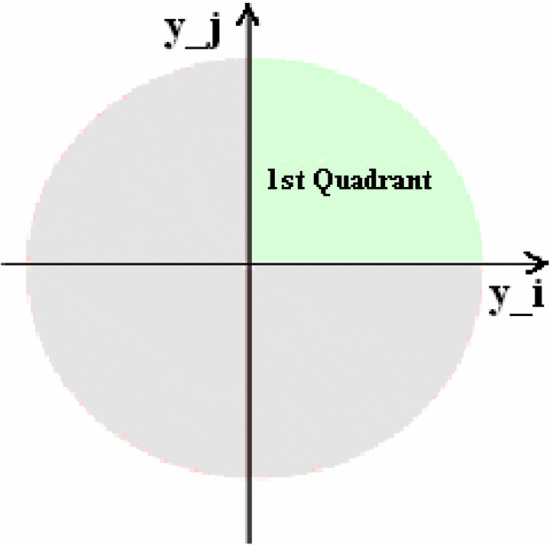
\includegraphics[scale=0.4]{report/images/quadrant.png}
    \caption{Figure showing first quadrant of cartesian cooredinate system \cite{kowalska2012maritime}}
    \label{fig:quad}
\end{figure}

.  Using this model they were able to perform motion prediction and using \emph{extreme value theory} anomaly detection.


\subsubsection{Neural Networks}
Neural Networks have become industry standard for most classification and regression tasks \cite{lathuiliere2018comprehensive}. They are able to achieve through the design of specific architectures to take advantage of the structure of the data they are trained on. For instance, Convolutional Neural Network's architectures are designed to use the 2 dimensional structure of images to learn spatial invariant features. This architecture design allows neural networks to outperform state-of-the-art in many computer vision tasks such as image classification \cite{krizhevsky2012imagenet, he2016deep} and object detection \cite{ren2015faster, he2016deep}. More relevant to our purposes however are Recurrent Neural Networks. These networks' architecture are instead designed to learn sequential invariant features in data. Resulting in exceptional performance in natural language generation \cite{wen2015semantically}, object tracking \cite{srivastava2015unsupervised} and trajectory prediction \cite{kim2017probabilistic}.

While a vanilla feed-forward neural network has the basic architecture of an input layer connected to one or more hidden layers, which are then connected to the output layer. Where between each layer the output of the previous layer is multiplied by a weight matrix $W$, then has a bias $b$ added to it, to be fed through an activation layer $\sigma$. Hence the output of layer j is given by the following equation:
$$g^j(\mathbf{x}) = \sigma(W_j\cdot g^{j-1}(\mathbf{x}) + b_j)$$
Where, $g^0(\mathbf{x})=\mathbf{x}$ (i.e. the activation layer of the input layer is the identity function.)

However, vanilla recurrent networks suffer from the vanishing/exploding gradient problem where if the gradient strays to far from 1 it either explodes or shrinks to zero during backpropagation. Thus, more intelligent architectures were constructed to be able to handle this problem.

Long Short Term Memory (LSTM) networks is an example of one of those architectures. To deal with the vanishing/exploding gradient problem LSTM's use gates that help it decide when to expose part of their cell state $C_t$ to the hidden state $h_t$. The idea being that some information in the cell state may not be relevant at every point in time. Thus, by only exposing it when needed, it reduces the amount of gradient multiplications during backpropagation that cause the vanishing/exploding gradient problem. See \citep{kawakami2008supervised} for a more detailed explanation.

\begin{figure}
    \centering
    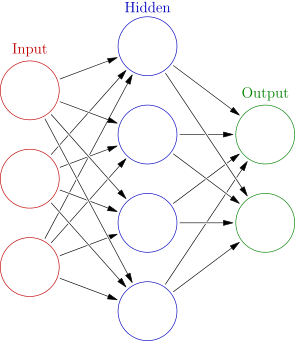
\includegraphics[scale=0.5]{report/images/Colored_neural_network.png}
    \caption{Figure showing architecture of vanilla neural networks. By Glosser.ca - Own work, Derivative of File:Artificial neural network.svg, CC BY-SA 3.0, \url{https://commons.wikimedia.org/w/index.php?curid=24913461}}
    \label{fig:vanilarch}
\end{figure}

Recurrent neural networks on the other hand as mentioned above have an architecture that takes advantage of sequences. Vanilla recurrent networks combines the information given from the input with a hidden state vector that they maintain. Where, the hidden state at time $t$ is given by:
$$h^t(\mathbf{x_t}) = \sigma( V \cdot h^{t-1}(\mathbf{x_{t-1}} + b_t) + U \cdot \mathbf{x_t})$$

\begin{figure}
    \centering
    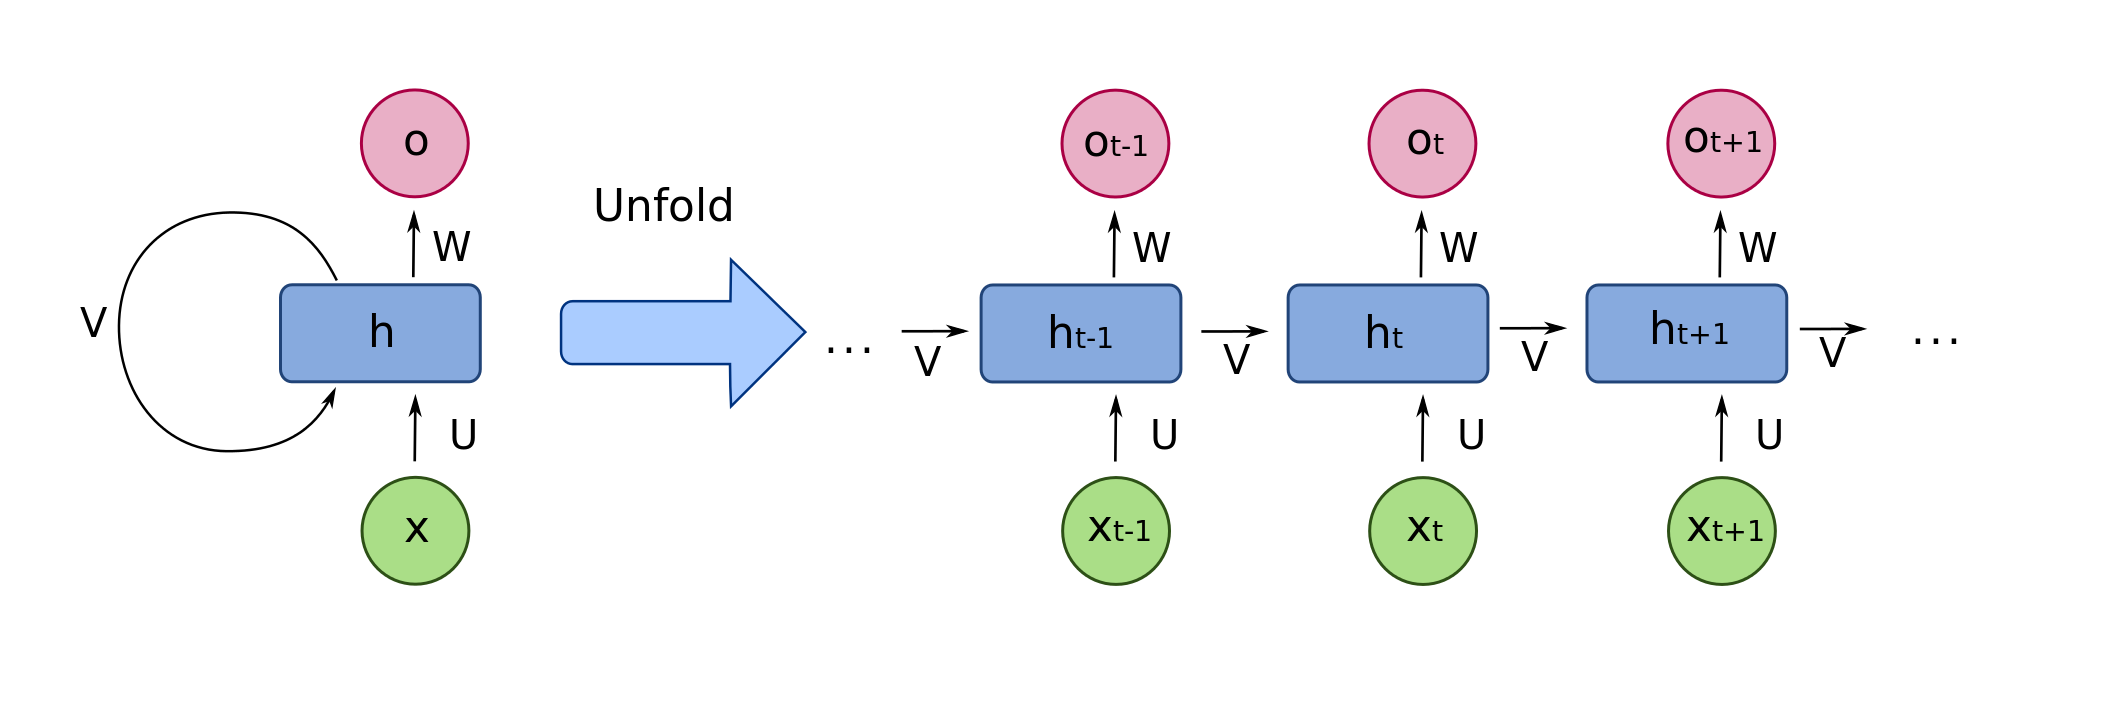
\includegraphics[width=\linewidth]{report/images/Recurrent_neural_network_unfold.png}
    \caption{Figure showing the unfolding of a recurrent neural network architecture. By François Deloche - Own work, CC BY-SA 4.0, \url{https://commons.wikimedia.org/w/index.php?curid=60109157}}
    \label{fig:my_label}
\end{figure}

Previous work in maritime surveillance even saw the use of recurrent neural networks. \citep{nguyen2018multi} used AIS data in a multi-task deep learning architecture for the purposes of trajectory reconstruction, anomaly detection and vessel type identification. In their paper the authors propose a variational recurrent neural network architecture which makes use of a h



\cite{pallotta2013vessel} used route prediction to assist in their anomaly detection system. They first extracted marine traffic routes using unsupervised clustering techniques. Then they used the extracted historical knowledge to develop probability models. One of the models gave a probability for the observed track of the vessel of interest and the corresponding temporal sequence given the suspected route the vessel it's on using a Hidden Markov Model which used a Weibull distribution for the state transition probability model and a Kernel Density Estimator for the evidence probability model. They also developed a prior probability model over routes by averaging the number of vessels that took those routes in the dataset. Using these probability models they developed a hypothesis test for anomaly detection.

\section{Technologies Used}
\label{sec:technologies}
A combination of C++ 14, Python and ROS was used to develop the system for this project. The core of the threat reaction system, which includes the control/ planning systems for agents, collision avoidance and detection system, and task allocation system. This was done because these systems need to operate at a high frequency, especially the task allocation system that has to forward simulate the environment for many samples at a high enough frequency to be useful. Furthermore, only the standard C++ libraries were used. Whereas, the threat detection system, simulation and visualisation were written in Python. This decision was made because the visualisation was easier to implement in Python and the threat-detection system uses Recurrent Neural Networks which are non-trivial to implement in C++. ROS was then used to communicate between the various systems each running in their own process. It was also used to model the concurrency that a real fleet of USV's would have to handle.

\subsection{\texttt{Python}}
\texttt{Python 3.6} was used for the simulation, analysis of the AIS data and for constructing and training the neural networks used for the intruder model. Table \ref{tab:pypack} lists the packages used and what they were used for. \texttt{Python 2.7} was used to interface with ROS through their rospy package. However, this caused challenges during implementation.

\begin{table}[]
\begin{tabular}{|l|l|}
\hline
\thead{Package}              & \thead{Use}                             \\ \hline
Matplotlib/ Searborn & Data analysis visualisation     \\ \hline
Tkinter              & Simulation Visualisation        \\ \hline
Sklearn              & Data analysis                   \\ \hline
Keras/ Tensorflow    & Neural Networks                 \\ \hline
Numpy                & Simulation/ Data Analysis/ Misc \\ \hline
\end{tabular}
\caption{List of python packages used and their uses}\label{tab:pypack}
\end{table}


\subsection{Robotics Operating System \texttt{(ROS)}}

As mentioned in \ref{sec:technologies}, we decided to use ROS for the communication between processes. In the coming section we describe how ROS works and how it assisted us in that task. Additionally, how it assisted us to organise the different subsystems into different packages built ontop one another. 

According to the ROS wiki \cite{roswiki} ROS is an open-source operating system for robots. Providing services commonly expected from an operating system, including but not limited to, hardware abstraction, message-passing between processes and package management. 

Furthermore, they mention that the ROS runtime "graph" is a peer-to-peer network of processes, which can potentially be distributed across multiple machines. ROS also implements several different styles of communication, including synchronous RPC-style communication over \textbf{services} \inlinecomment{TODO ref services}, asynchronous streaming of data over~\textbf{topics}, and storage of data on a Parameter Server. These styles of communication were all necessary and used in this project. 

\subsubsection{Nodes}
\label{def:node}
A node, as defined by the wiki~\cite{roswiki}, is a process that performs computation. Nodes are combined together into a graph and communicate with one another using streaming topics~\ref{def:topic}, RPC services~\ref{def:serv}, and the parameter server. The nodes in ROS provide several benefits to the overall system such as fault tolerance as crashes are isolated to individual nodes. This provides a robustness that is needed for real-world applications.

\subsubsection{Topics}
\label{def:topic}
The wiki \cite{roswiki} describes topics as named buses over which nodes exchange messages. Thus, if a node is interested in data passing over a specific topic, it can subscribe \ref{def:sub} to that topic and get that data. If a node generates data it can share this data with other nodes by publishing \ref{def:pub} to a relevant topic. 

\subsubsection{Messages}
\label{def:sub}
Each topic is strongly typed by the ROS message type used to publish to it and nodes can only receive messages with the matching type. These messages also function as the actual container for the data following a simplified message description language.

Each field consists of a type and a name, separated by a space, i.e:
%TODO ROS MESSAGES

The messages used in this project can be found in the \emph{swarm\_msgs} package.

\subsubsection{Publishers}
\label{def:pub}
Publishers are what nodes use to advertise and then share what data they want to share under a specific topic.

\subsubsection{Subscribers}
Subscribers are what nodes use to listen to data being passed under a certain topic. When a node subscribes to a topic it is letting the \emph{rosmaster} know that whenever a message is published under a specific topic that it would like to react to that message. It reacts to the messages by providing the subscriber with a callback function that is called whenever a new message is published for the purpose of processing that message.

\subsubsection{Services}
\inlinecomment{TODO}

\subsubsection{Parameter Server}
\inlinecomment{TODO}


\subsubsection{Package Structure}
The different subsystems are organised into the following packages:
\begin{itemize}
	\item swarm\_core
	\item swarm\_msgs
	\item swarm\_control
	\item swarm\_task\_manager
	\item swarm\_planner
	\item swarm\_threat\_detection
\end{itemize}
The dependencies of these packages can be seen in \ref{img:packages} with the relevant packages highlighted in red.

\begin{figure}
    \centering
    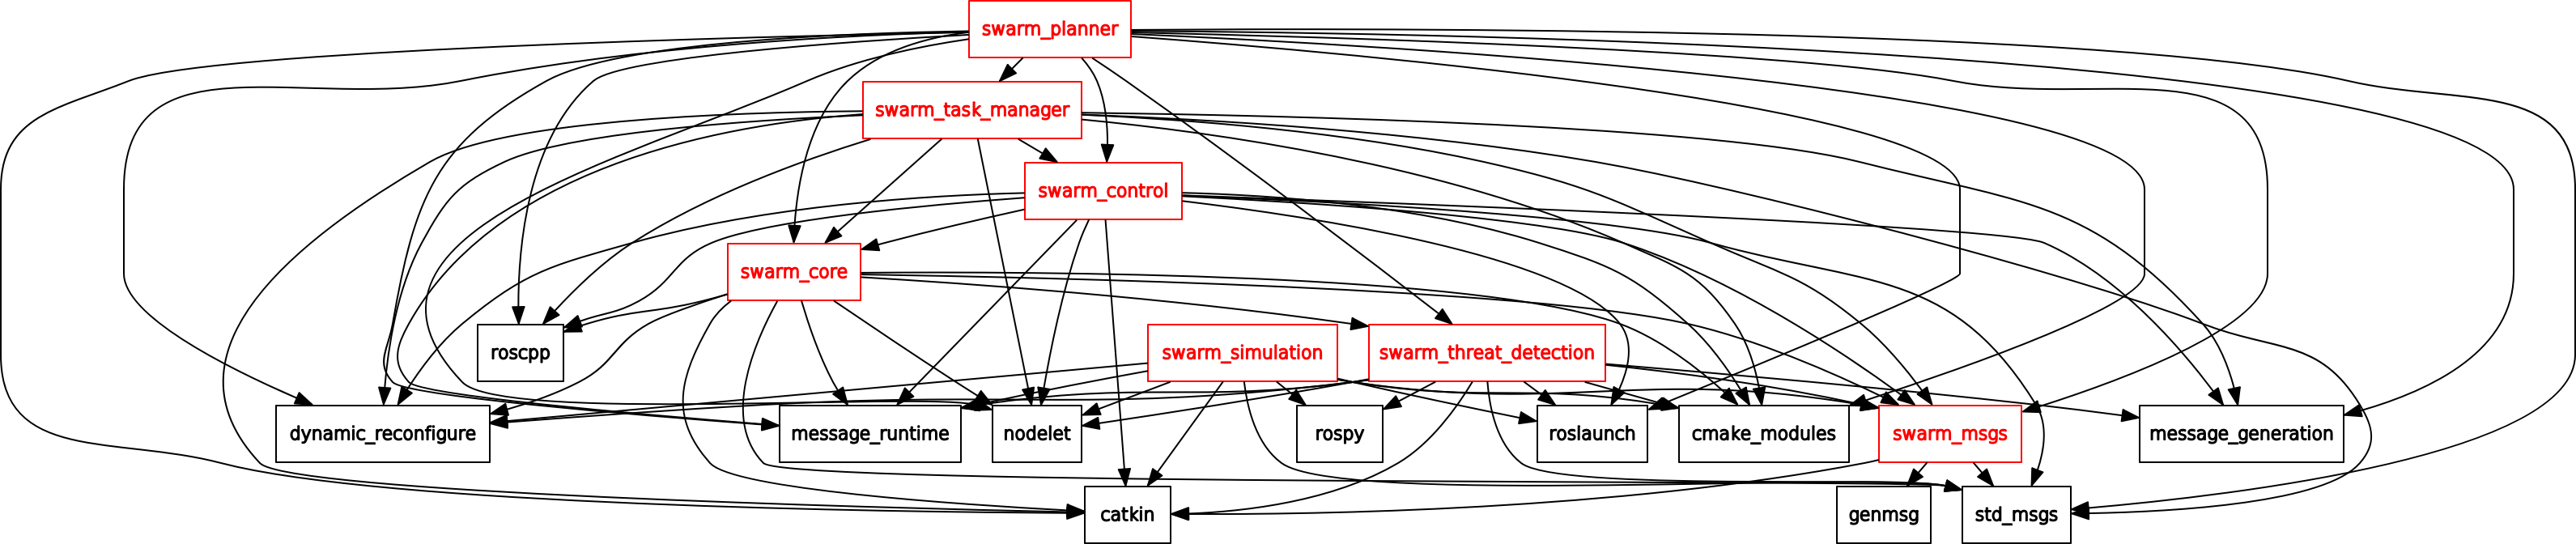
\includegraphics[width=\linewidth]{report/images/rospackgraph.png}
    \caption{Graph showing dependencies of packages}
    \label{img:packages}
\end{figure}


\chapter{Vessel Traffic Model}
\label{chap:model}
In this chapter we describe in detail, the vessel traffic model we used to simulate benign vessels. Additionally, we describe the Automated Identification System (AIS) dataset that the model was trained on. Specifically, we describe how we preprocess the data to train our model, and the challenges that came with it. Furthermore, we also compare and contrast our model to previous work on modelling vessel traffic.

\section{Automated Identification System (AIS)}
\label{sec:ais}
The Automated Identification System (AIS) provides means for ships ships to electronically broadcast ship data including: vessel identification, position, course, and speed at regular intervals \citep{perez2009automatic}. Vessels equipped with these transceivers broadcast their data over 162 ± 0.25 MHz radio frequency (VHF), to be captured by other vessels, terrestrial receivers or the AIS satellite network. These are then given to Maritime Data Providers like \href{https://maritimeintelligence.informa.com/}{maritime intelligence} and \href{https://marinecadastre.gov/ais/}{marine cadastre} to be decoded, stored and shared. For this project we used \href{https://marinecadastre.gov/ais/}{marine cadastre's} free and publicly available dataset gathered through the United States Coast Guard's \href{https://www.navcen.uscg.gov/?pageName=NAISmain}{national network} of AIS receivers. Their dataset is split into UTM zones and by the month and year, but for our purposes we focused only the vessel traffic for the whole year of 2017 in the 18th UTM zone. To download the dataset, we scrapped directly from their website using the \href{https://www.gnu.org/software/wget/}{\textbf{wget}} command as they describe on their \href{https://coast.noaa.gov/htdata/CMSP/AISDataHandler/2017/index.html}{website}. However, because the zipped the entire dataset was approximately 10GB and 40GB unzipped, we had to find non-trivial ways to load the data for preprocessing \ref{sss:pipeline}.

\begin{figure}
    \centering
    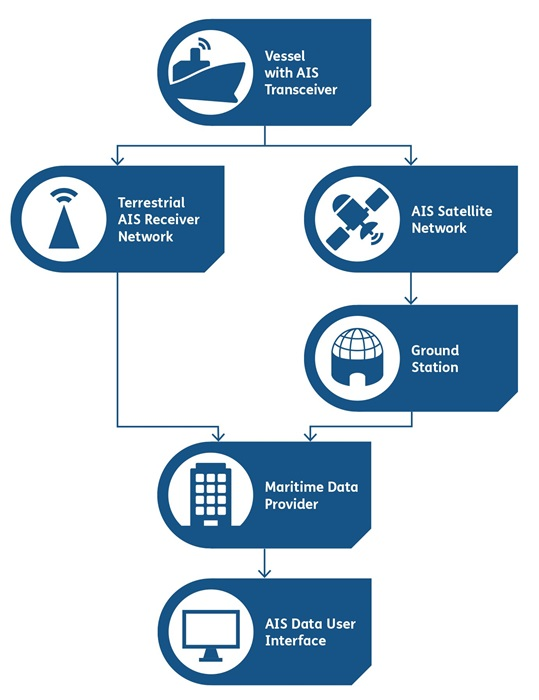
\includegraphics[scale=0.8]{report/images/Understanding_AIS_Fig1.jpg}
    \caption{Figure showing the terrestrial and satellite AIS data routing map sourced from \href{https://maritimeintelligence.informa.com/}{marine intelligence} }
    \label{fig:my_label}
\end{figure}

\subsection{Dataset Description}
The dataset \href{https://marinecadastre.gov/ais/}{marine cadastre} provides contains records for U.S. coastal waters for the calender years 2009-2017. They are filtered to one minute intervals and formatted in zipped monthly files by Universal Transverse Mercator (UTM) zone (A map of the different UTM zones are shown in figure \ref{fig:utm}). Ship names and call sign fields were removed and the Maritime Mobile Service Identity (MMSI) for each has been encrypted. We present the columns of the dataset with a short description in table \ref{tab:cols}. However, we could not find descriptions for the Draft and Cargo columns.

Out of the columns presented, we focused only  on the following relevant columns:
\begin{itemize}
    \item MMSI
    \item BaseDateTime
    \item Lat
    \item Lon
    \item SOG
    \item Heading
    \item COG
    \item VesselType
\end{itemize}

\begin{table}[]
\begin{tabular}{|l|l|}
\hline
\thead{Column}       & \thead{Description}                                                  \\ \hline
MMSI         & Maritime Mobile Service Identity number of the vessel                        \\ \hline
BaseDateTime & Date/time string in "yy-mm-dd-hh-mm-ss" format                               \\ \hline
LAT          & Latitude geocoordinate of vessel                                             \\ \hline
LON          & Longitude geocoordinate of vessel                                            \\ \hline
Heading      & Vessel's heading                                                             \\ \hline
COG          & Vessel's course over ground                                                  \\ \hline
SOG          & Vessel's speed over ground                                                   \\ \hline
Vessel Name  & Name of the vessel                                                           \\ \hline
IMO          & International Maritime Organisation number of the vessel                     \\ \hline
CallSign     & Call sign of the vessel                                                      \\ \hline
Vessel Type  & Numeric identifier of vessel type                                            \\ \hline
Status       & Current status of vessel (e.g. anchored, moored, under way etc.)             \\ \hline
Width        & Width of vessel                                                              \\ \hline
Draft        & No Description Found                                                         \\ \hline
Cargo        & No Description Found                                                         \\ \hline
\end{tabular}
\caption{Table of the columns of the dataset with a short description.}\label{tab:cols}
\end{table}

\begin{figure}
    \centering
    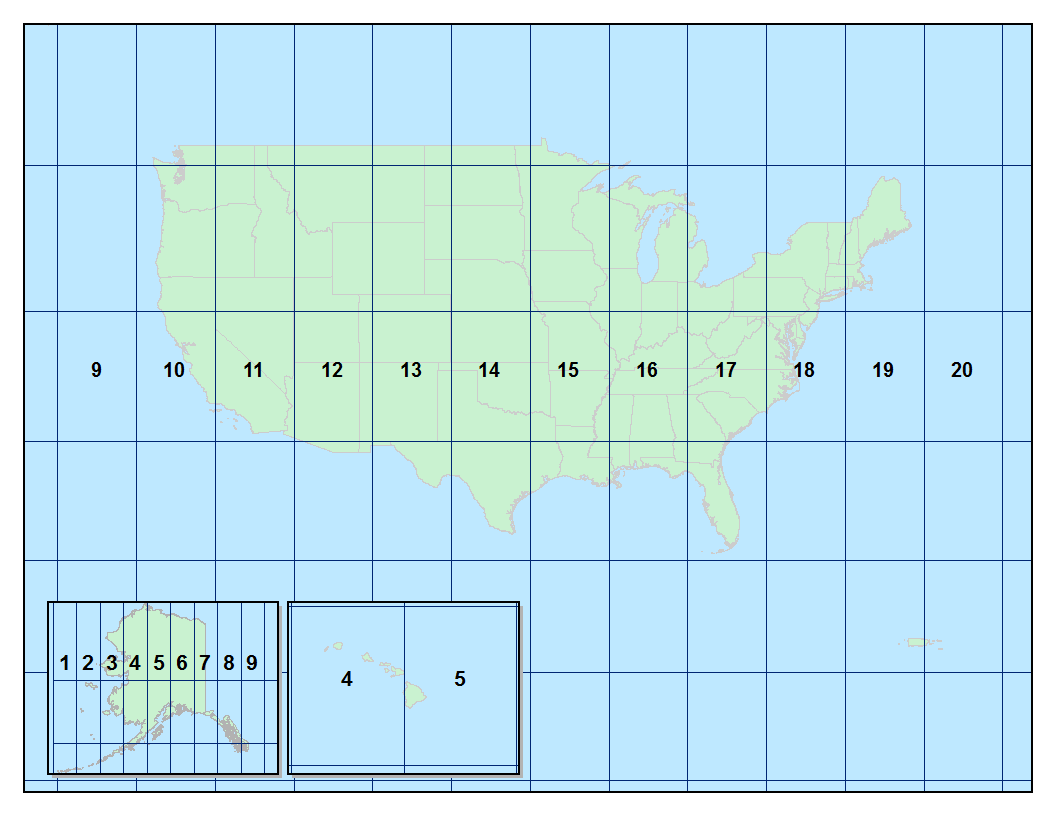
\includegraphics[width=0.8\linewidth]{report/images/UTMZoneMap2014.png}
    \caption{UTM zone map.}
    \label{fig:utm}
\end{figure}

\subsection{Preprocessing}

\subsubsection{Cleaning}
\label{sss:cleaning}
Firstly, all the rows which with \emph{Nans} were dropped. We could afford to do this because, there were not that many of them compared to the size of the dataset. Then using marine cadastre's \href{}{visualisation tool} we narrowed down the area of interest to the data with latitudes in the region (36.7, 37.0) and latitudes within the region (-76.8733, -75.60036). We made this decision because it was easier to see the vessel behaviour and the models performed better when trained on the reduced region rather than the larger region. We also focused on the vessels of vessel type 1004, 1025 and 1024 because these were the three most common vessel types in the dataset. These vessel types correspond to Cargo, Tanker and Tug Tow vessels. Data points with SOG lower than 0.5 were also removed because we are more interested in dynamic rather than stationary behaviour of vessels.

\subsubsection{Geocoordinates to Cartesian Coordinates}
\label{sss:geo}
Longitude and latitude when combined with altitude form spherical coordinates. These coordinates can be used to position you anywhere in the world and are commonly used to represent a vehicles positions in land, sea or air. However, they cannot be used for kinematic calculations directly because they are in a different coordinate system. Hence, we had to convert it from the spherical geocoordinates to a standard cartesian coordinates. To do this conversion, you need a longitude latitude point to act as the centre, and we chose (-75.8733, 36.9195) as the centre. Firstly, we calculate the bearing between points to be transformed and the centre point, using the spherical law of cosines. We then calculate distance between the two points, using the haversine distance which is a common approximation for the distance between two longitude-latitude points. Using the bearing, the distance from the centre and the centre we set up a standard cartesian coordinate frame centred at the chosen centre point. The exact mathematical equations are given below.

\begin{align*}
    \theta &= \acos(\sin\phi_c \cdot \sin\phi + \cos\phi_c \cdot \cos\Delta\lambda) \\
    a &= \sin^2\big(\frac{\Delta\phi}{2}\big) + \cos \phi_c \cdot \cos \phi \cdot \sin^2\big(\frac{\Delta\lambda}{2}\big) \\
    c &= 2 \atan(\sqrt{a}, \sqrt{1-a}) \\
    r &= R\cdot c \\
    x &= r\cos{\theta} \\
    y &= r\sin{\theta} \\
\end{align*}
where,

\hspace{0.25in} $(\phi_c, \lambda_c)$ \text{is the longitude-latitude centre point}

\hspace{0.25in} $(\phi, \lambda)$ \text{is the longitude-latitude point to be transformed}

\hspace{0.25in} $R$ \text{is the earth's radius in km}

\hspace{0.25in} $\theta$ the bearing between the two points from the spherical law of cosines

\hspace{0.25in} $r$ the distance between the two points from the haversine distance.

\hspace{0.25in} $(x, y)$ the point in cartesian coordinates in km units.

\subsubsection{Smoothing}
\label{sss:smoothing}
A very important feature needed by our model is the heading of the vessels. Unfortunately, the headings recorded in the environment appeared to be unreliable. Firstly, many rows had a heading simply set to 500, which doesn't make intuitive sense for an angle. Furthermore, upon further inspection of the data, we would saw odd readings for the reported headings, like what's displayed in figure \ref{fig:badheadings}. Hence, we decided instead to use the angle between every consecutive trajectory position and use that as the heading estimate. However, as you can see in \ref{fig:headings} this can be pretty noisy especially when there are jumps in the data. To solve this problem we decided on using a passing filter. In figure \ref{fig:filters} you can see us testing different windows and window sizes. Eventually, we settled on using the \emph{hanning} window with a window size of 21. After smoothing the heading and speed are used to construct smoothed velocity vectors like the ones seen in \ref{fig:headings}

\begin{figure}
    \centering
    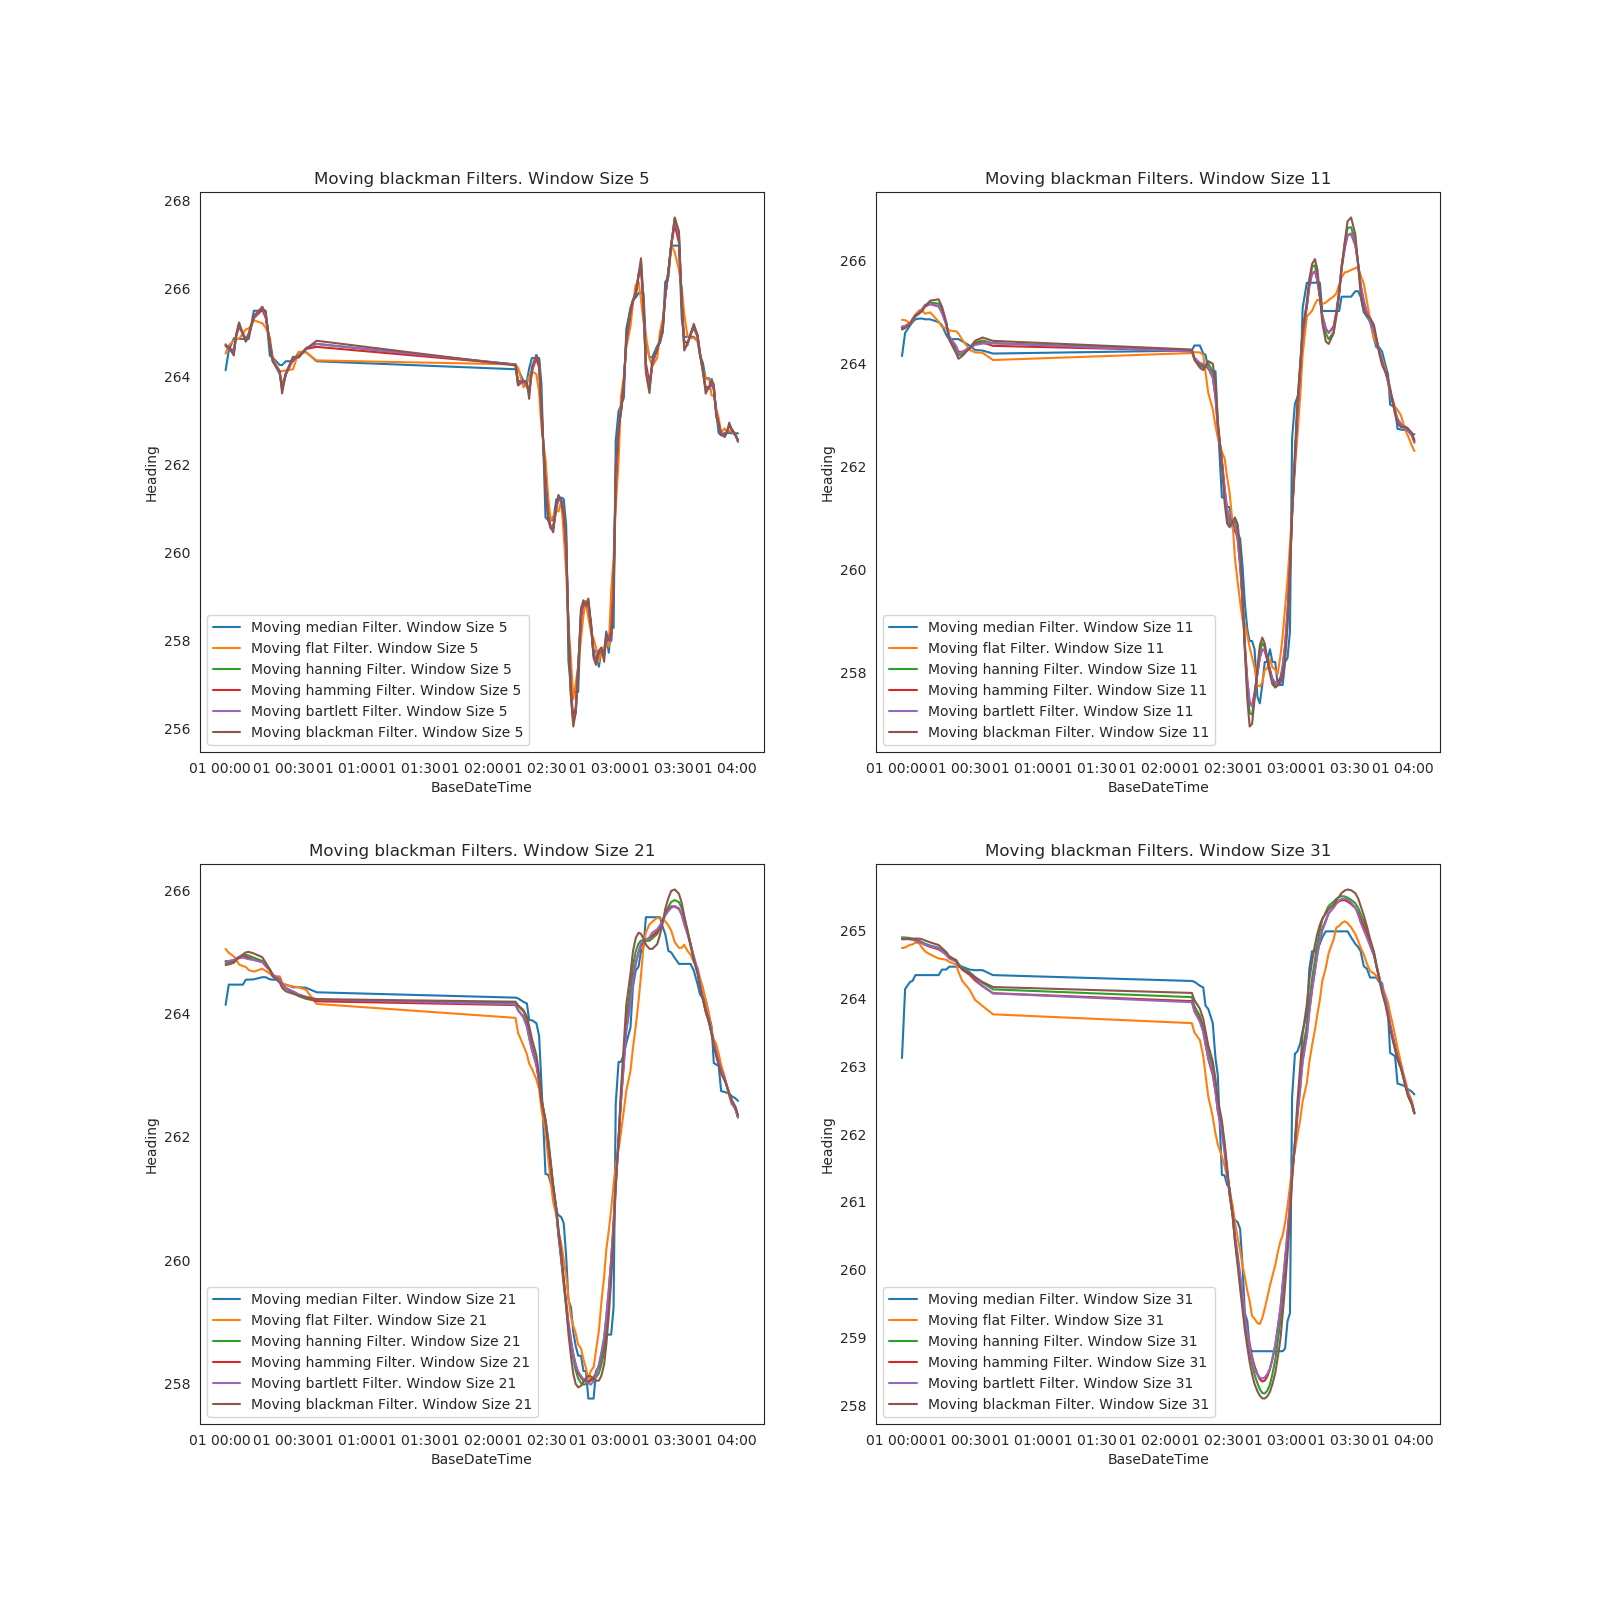
\includegraphics[width=\linewidth]{report/images/filters.png}
    \caption{Figure showing the effects of different filters with different filter sizes on smoothing the point-wise heading}
    \label{fig:filters}
\end{figure}

\begin{figure}
    \centering
    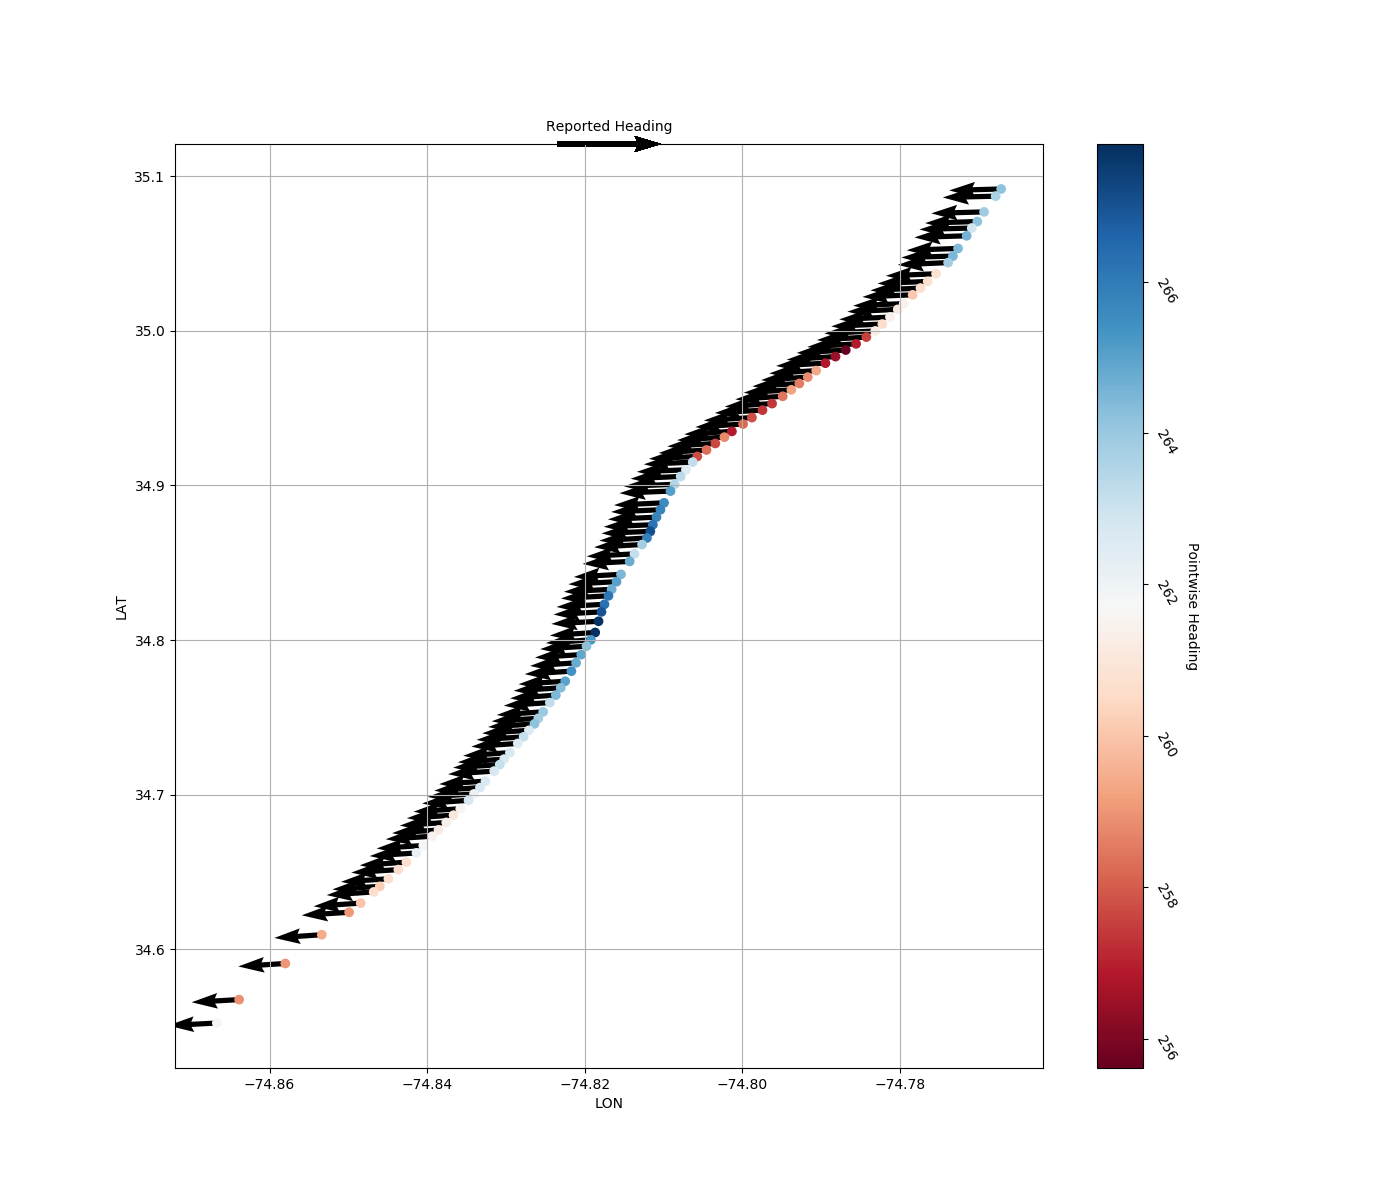
\includegraphics[width=\linewidth]{report/images/badheadings.png}
    \caption{Figure showing trajectory of vessel with arrows showing the reported heading at that point. Points are highlighted according the point-wise heading at that point.}
    \label{fig:badfigures}
\end{figure}

\begin{figure*}
    \centering
    %\begin{subfigure}
        \centering
        \subfigure[\texttt{Reported}]{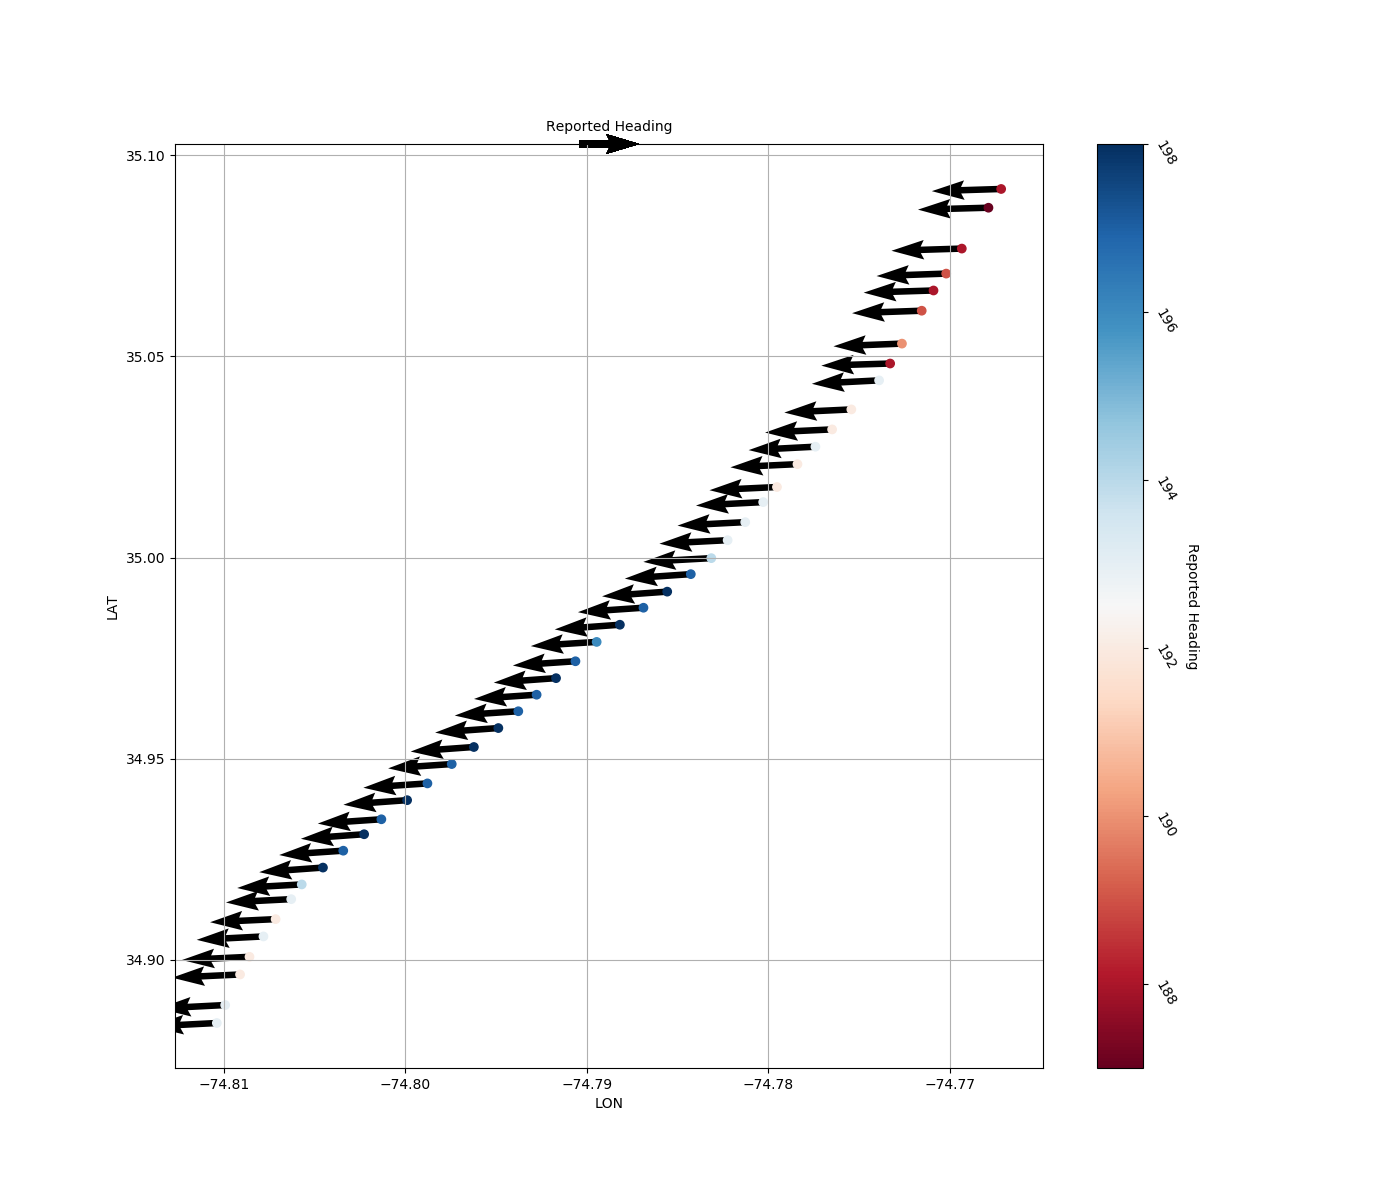
\includegraphics[width=0.45\linewidth, height=2in]{report/images/reportedheadings.png}}
        %\caption*{\texttt{Tanker}}\label{fig:tanker}
    %\end{subfigure}
    % \hfill
        \subfigure[\texttt{Point-wise}]{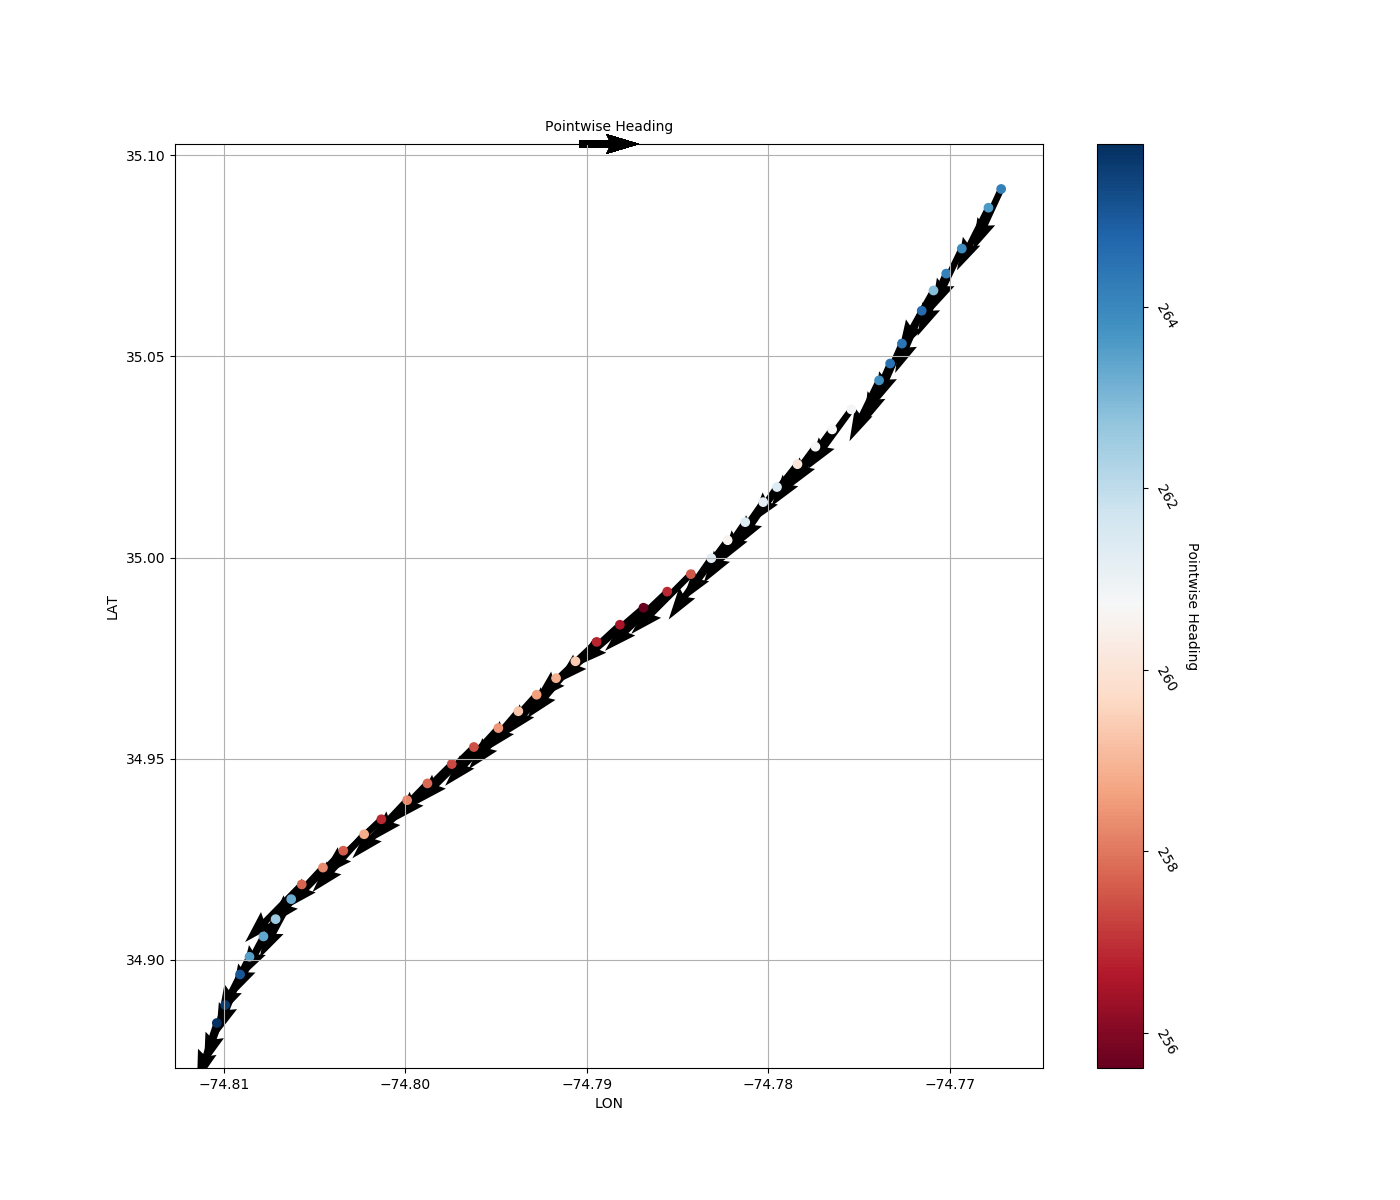
\includegraphics[width=0.45\linewidth, height=2in]{report/images/pointwiseheadings.png}}
        %\caption*{\texttt{Oil platform} }\label{fig:oil}
    % \hfill
        \subfigure[\texttt{Smoothed}]{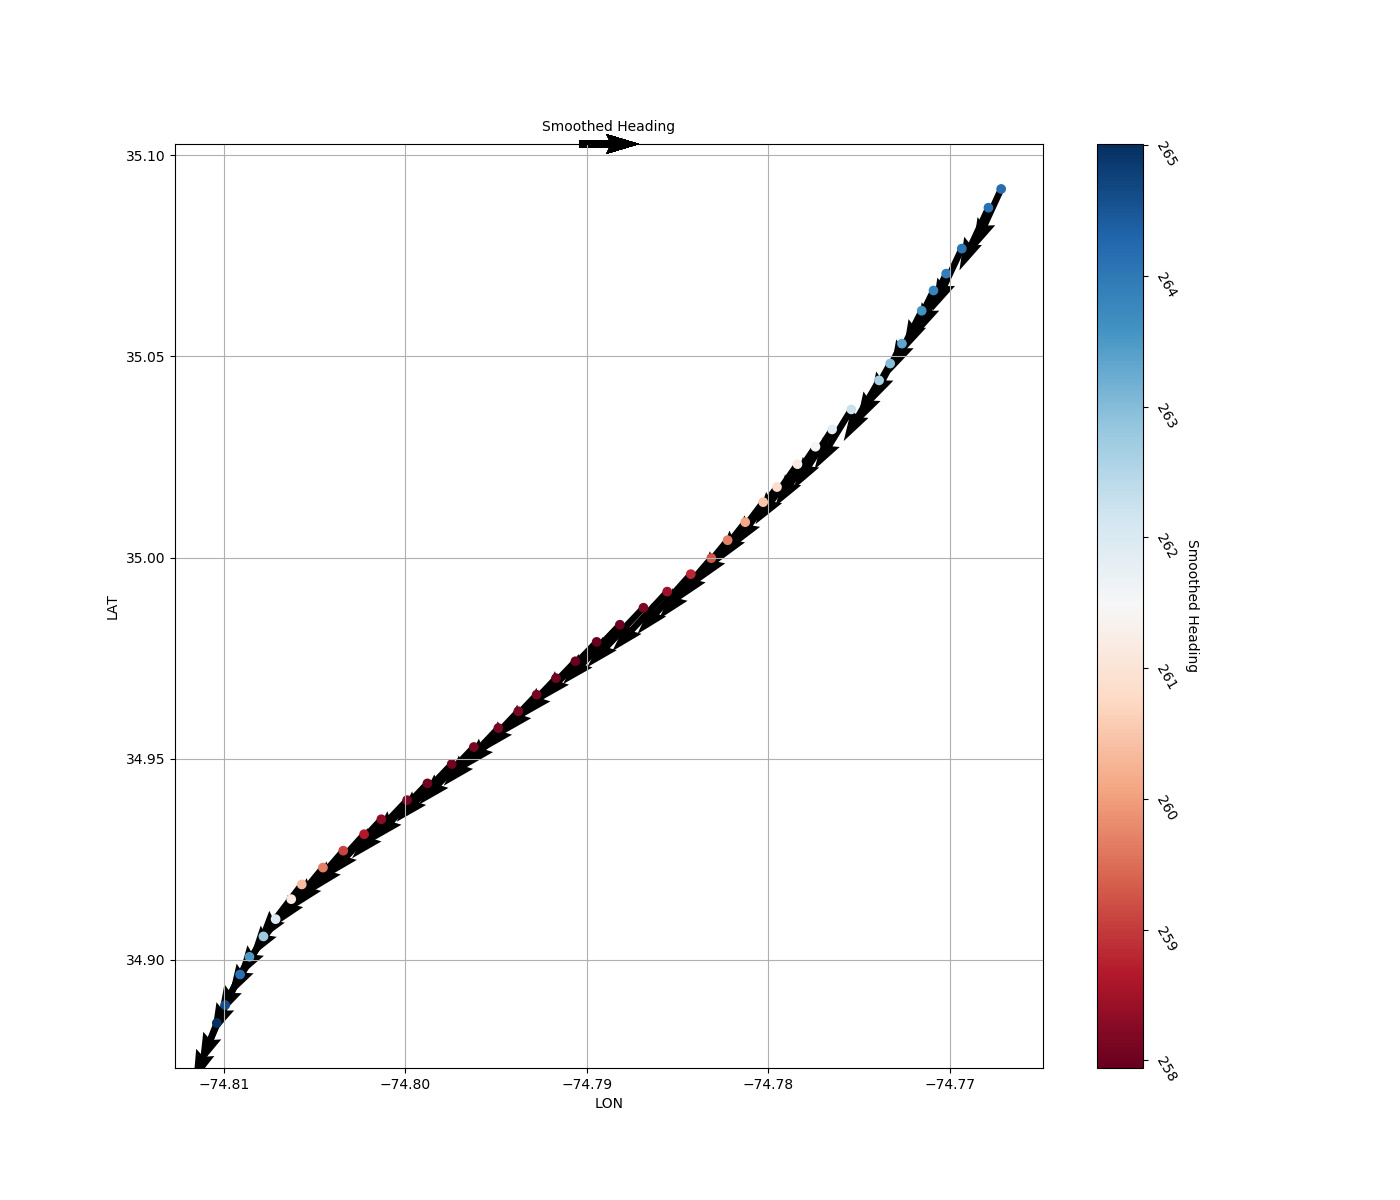
\includegraphics[width=0.8\linewidth, height=2in]{report/images/smoothedheadings.png}}
        %\caption*{\texttt{Oil platform} }\label{fig:oil}
    
    \caption{Figure displaying (a) Reported (b) Point-wise and (c) Smoothed Headings for a vessel trajectory}\label{fig:headings}
\end{figure*}

\subsubsection{Preprocessing Pipeline}
\label{sss:pipeline}
As mentioned above in \ref{sec:ais} the dataset adds up to larger than 40 GBs, causing any standard computer to run out of memory if loaded naively. To solve this problem we made use of \textbf{pandas} \texttt{read\_csv} which has a \texttt{chunksize} parameter. This parameter allows you to iteratively load the dataset in chunks instead of all at once. Thus, our preprocessing pipeline went as the following:

\begin{itemize}
    \item Load dataset into memory, 100000 rows at a time.
    \item Drop any nan's or rows with missing values.
    \item Drop data outside the longitude-latitude boundaries. mentioned in \ref{sss:cleaning}
    \item Convert lon-lat points to points in cartesian coordinate frame \ref{sss:geo}.
    \item Append processed chunk to previously processed data.
    \item Once all the chunks have been loaded and processed. Sort data by BaseDateTime column so that points are in consecutive order.
    \item Calculate pointwise headings, smooth them and use them to construct smoothed velocity vectors \ref{sss:smoothing}.
\end{itemize}

\subsection{Analysis and Visualisation}
\begin{figure}
    \centering
    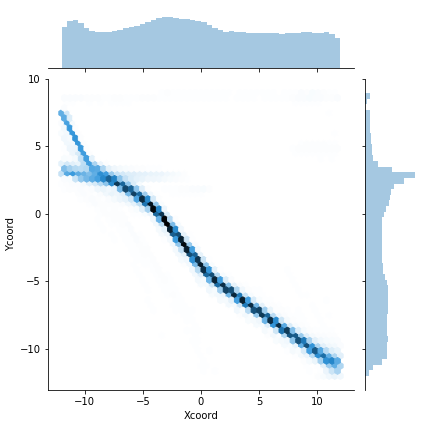
\includegraphics[scale=0.8]{report/images/latlonhex.png}
    \caption{Hex plot showing distribution of vessel trajectories in area of interest}
    \label{fig:my_label}
\end{figure}

\begin{figure}
    \centering
    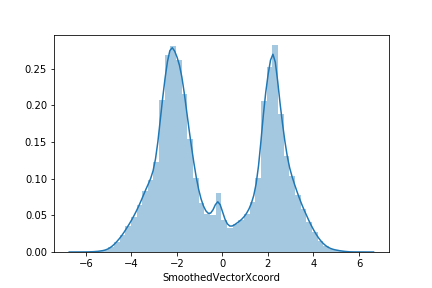
\includegraphics[scale=0.6]{report/images/vectorxhist.png}
    \caption{Bi-modal distribution plot of SmoothedVectorX}
    \label{fig:distx}
\end{figure}

\begin{figure}
    \centering
    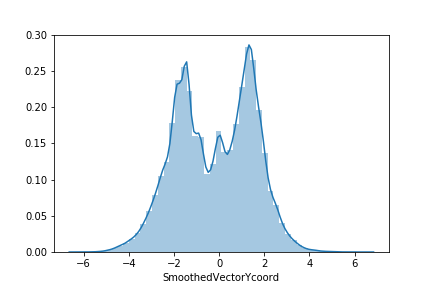
\includegraphics[scale=0.6]{report/images/vectoryhist.png}
    \caption{Bi-modal distribution plot of SmoothedVectorY}
    \label{fig:disty}
\end{figure}

\begin{figure}
    \centering
    \subfigure[SmoothedVectorX]{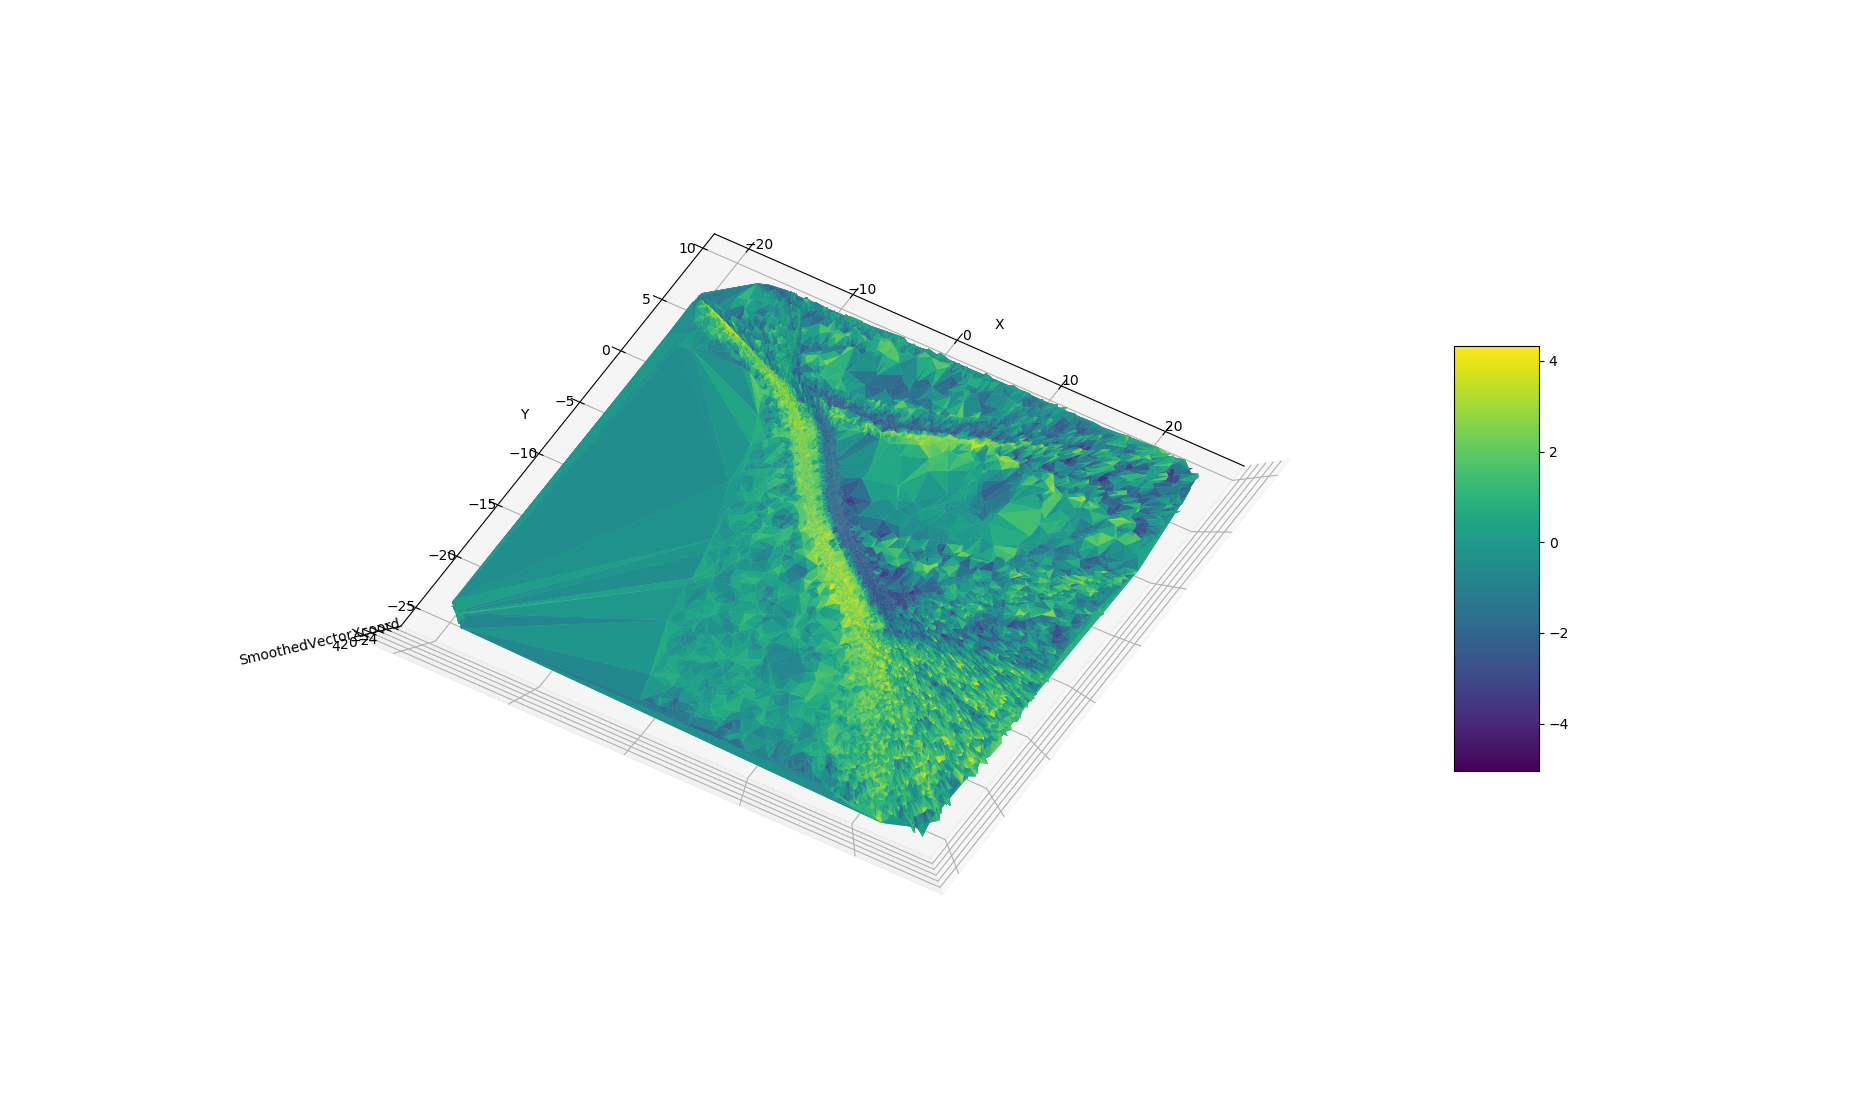
\includegraphics[width=0.45\linewidth]{report/images/vecx3d.png}}
    \subfigure[SmoothedVectorY]{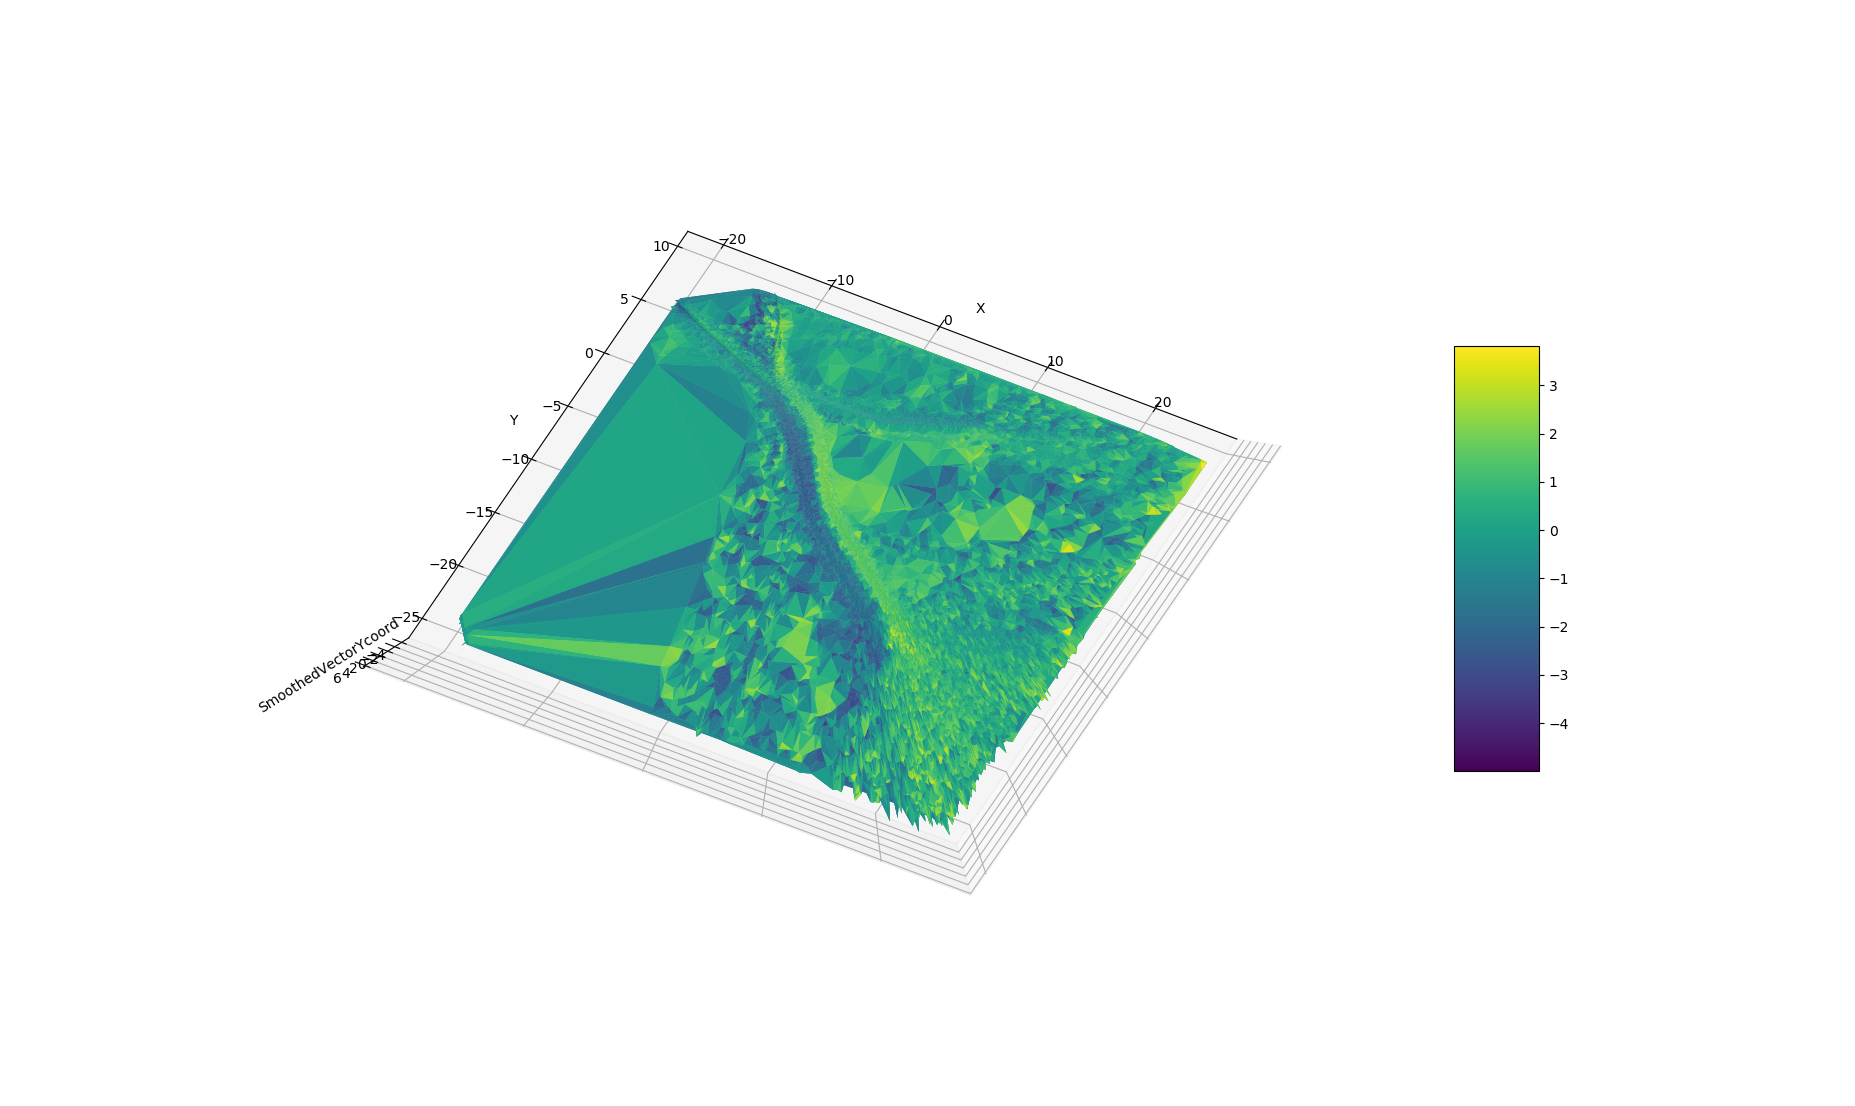
\includegraphics[width=0.45\linewidth]{report/images/vecy3d.png}}
    \caption{Top down view of surface plot of vector coordinates on the z-axis and x and y coordinates on their respective axes}
    \label{fig:surface3d}
\end{figure}

\section{Model}

To be able to model vessel traffic, we designed a model that predicts the vessel's kinematics given it's previous positions.
$$P(\dot{x_t}, \dot{y_t}| x_{0..t}, y_{0..t})$$
Where the kinematics of the vessel describes the vessel's motion without external forces. Which for our purposes is the vessel's velocity. As a deviation from most previous work in this area, we will not take vessel types into account in our model. This decision was made because, we are research focus is closer to that of manoeuvre onset detection \ref{} (e.g. taking a drastic turn towards the asset) rather than suspicious behaviour like a vessel suddenly slowing down, or a vessel of a particular type being somewhere it isn't normally. Those are interesting topics in themselves and could be an example of further research beyond this project.

Initially, we considered using Gaussian Processes much in the same way \citep{kowalska2012maritime} did. However, as mentioned in \ref{chap:background} it would only be able handle unimodal data and thus, it could only model boats following one trade route going in one direction. Also, gaussian processes like other kernel models are expensive to use for prediction, especially for large training sets. This would become a problem because our model needs to be able to run at at least 10Hz. Then we thought about using basic feed-forward neural networks, however they were giving sub par performance. We hypothesised that this was because the kinematics could not be directly determined given just the current positions. Though, this could possibly be solved by including the kinematics of the previous state. However, as i.e. $P(\dot{x_t}, \dot{y_t}| x_{0..t}, y_{0..t}) \not\approx P(\dot{x_t}, \dot{y_t}| x_{t}, y_{t})$. \inlinecomment{TODO This might have been fixed by adding the previous state's kinematics to the input.}We finally settled on using a recurrent neural network with LSTM cells after is showed much performance than the other models. Also, after the model selection experiments described in \inlinecomment{TODO ref experiments} we settled on a recurrent network with 128 LSTM cells, which takes a sequence of 10 normalised position coordinates in km and outputs the estimated velocity of the vessel in m/s.

\chapter{Threat Detection System}
\label{chap:detection}
\section{Manoeuvre onset detection}
\section{Threat probability}
\chapter{Threat Reaction System}
\label{chap:reaction}
\section{Swarm Core}
In this section we introduce the notion of an agent and the types of agents used in this project. Furthermore, we introduce and define tools that will be used by the agents in this and the future sections. 

\subsection{Agents}
\label{def:agent}
An \textbf{agent}, as defined by \citet*{russell2016artificial}, is something that perceives and acts in an environment. Furthermore, they define and describe four different types of agents. The descriptions of which can be found in \ref{tab:agents}. These definitions become useful when describing the agents used in our system.

\begin{table}[]
\begin{tabular}{|l|l|}
\hline
\thead{Agent}                     & \thead{Description}                                                                                         \\ \hline
Simple reflex agents      & These directly respond to percepts.                                                                 \\ \hline
Model-based reflex agents & \makecell[l]{These maintain an internal state and track aspects \\ of the world
not evident in the current percept.} \\ \hline
Goal-based agents         & These act to achieve their goals.                                                                   \\ \hline
Utility-based agents      & These agents try to maximize their own expected happiness.                                          \\ \hline
\end{tabular}
\caption{Table of Agent descriptions}\label{tab:agents}
\end{table}

\subsubsection{Asset Agent}
This is the agent the USV's \ref{def:usv} are tasked with protecting. This agent can be thought of as a dynamic tanker vessel moving along a predefined route or a stationary oil rig. In previous works \cite{}\cite{} this agent has been both stationary and dynamic. However, for the purpose of this system, the agent has been set to remain stationary. This decision was made due to time constraints, and the fact that previous work \cite{} showed that this didn't lead to more exciting results. That being said, it can be easily shown how the techniques used can generalise to a dynamic asset. Because the asset is fixed and doesn't react to anything in the environment,  it trivially falls in the simple-reflexive agent category.

\begin{figure*}
    \centering
    %\begin{subfigure}
        \centering
        \subfigure[\texttt{Tanker}]{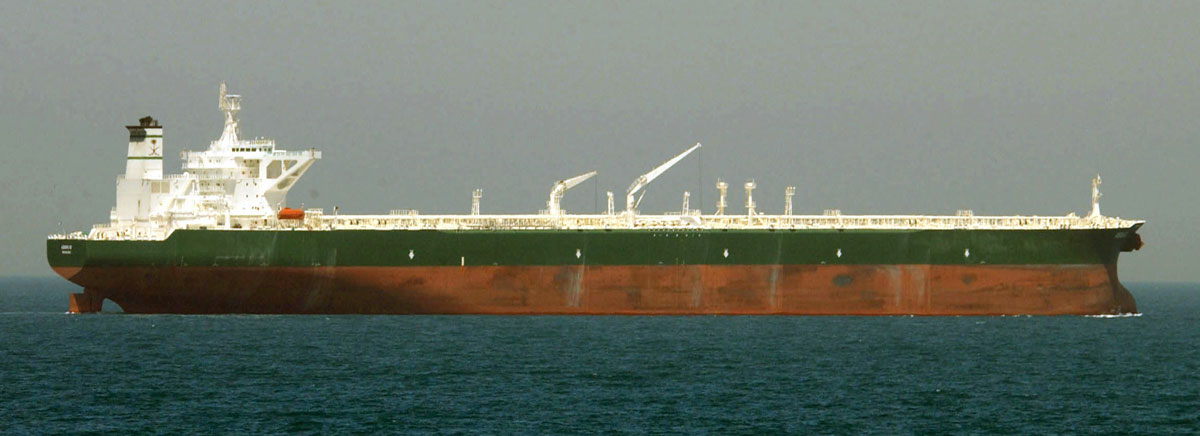
\includegraphics[width=0.6\linewidth, height=1in]{report/images/tanker.jpg}}
        %\caption*{\texttt{Tanker}}\label{fig:tanker}
    %\end{subfigure}
    \hfill
        \subfigure[\texttt{Oil platform}]{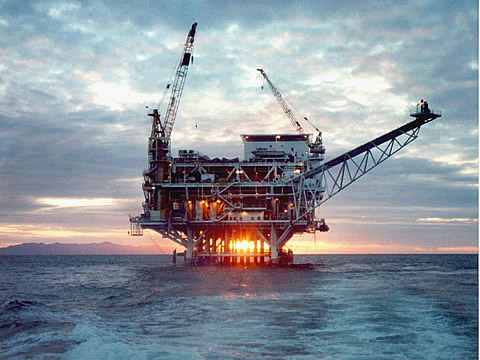
\includegraphics[width=0.3\linewidth, height=1in]{report/images/oilrig.jpg}}
        %\caption*{\texttt{Oil platform} }\label{fig:oil}
    \caption{Figure displaying (a) Tanker \citep{crudepict2005} and (b) Oil Platform \citep{oilpict2005}}
\end{figure*}

\subsubsection{Intruder Agent}
\label{def:intruder}
\textbf{Intruder agents} are defined as agents that have come within a \textit{suspicious} radius of the \textbf{asset agent}. This can be because of benign reasons such as a vessel following a common trade route. However, it could be because of more malicious reasons. This is why the intruder agents are split into two categories, malicious and benign. A \textbf{benign intruder agent} is just a normal vessel following a common trade route. This agent is also equipped with a collision detection and reaction system but doesn't have a predefined goal. Instead its behaviour is described by the learned model described in \inlinecomment{Cite Model}. Because this agent has no particular goal it wants to achieve, or utility it wants to maximise it can also be classified as a simple-reflexive agent. On the other hand, a \textbf{malicious intruder} is displays a different behaviour than that of a \nonthreat intruder agent. For the purposes of this project, we assume intruder agents are assumed to have one goal, \textbf{reach the asset}. This was also an assumption taken by \citet{raboin2013model} and \citet{moundegue2017fields}. However, like \citet{raboin2013model} we assume that intruders can also pretend to be benign displaying normal vessel behaviour before eventually switching to malicious behaviour. This goal-oriented behaviour earns threat-intruder agents the classification of goal-based agents.

\subsubsection{Unmanned Surface Vehicles (USV) Agents}
\label{def:usv}
Unmanned Surface Vehicles commonly referred to as USV's are defined as autonomous vehicles that operate on the surface of a body of water. For purposes of this project, we assume that the threat reaction system is given a fleet of heterogeneous USVs with different kinematic constraints. Each of these USV's is equipped with the same set of behaviours \ref{sec:behaviours} which they use to delay threat-intruder agents for as long as possible. Hence, the threat reaction system can be viewed as a multi-agent system where the agents are trying to maximise a common utility. This utility is the amount of time they can delay intruder's before they reach the asset. Thus, the USV agents can be considered utility-based agents.

\begin{figure}
    \centering
    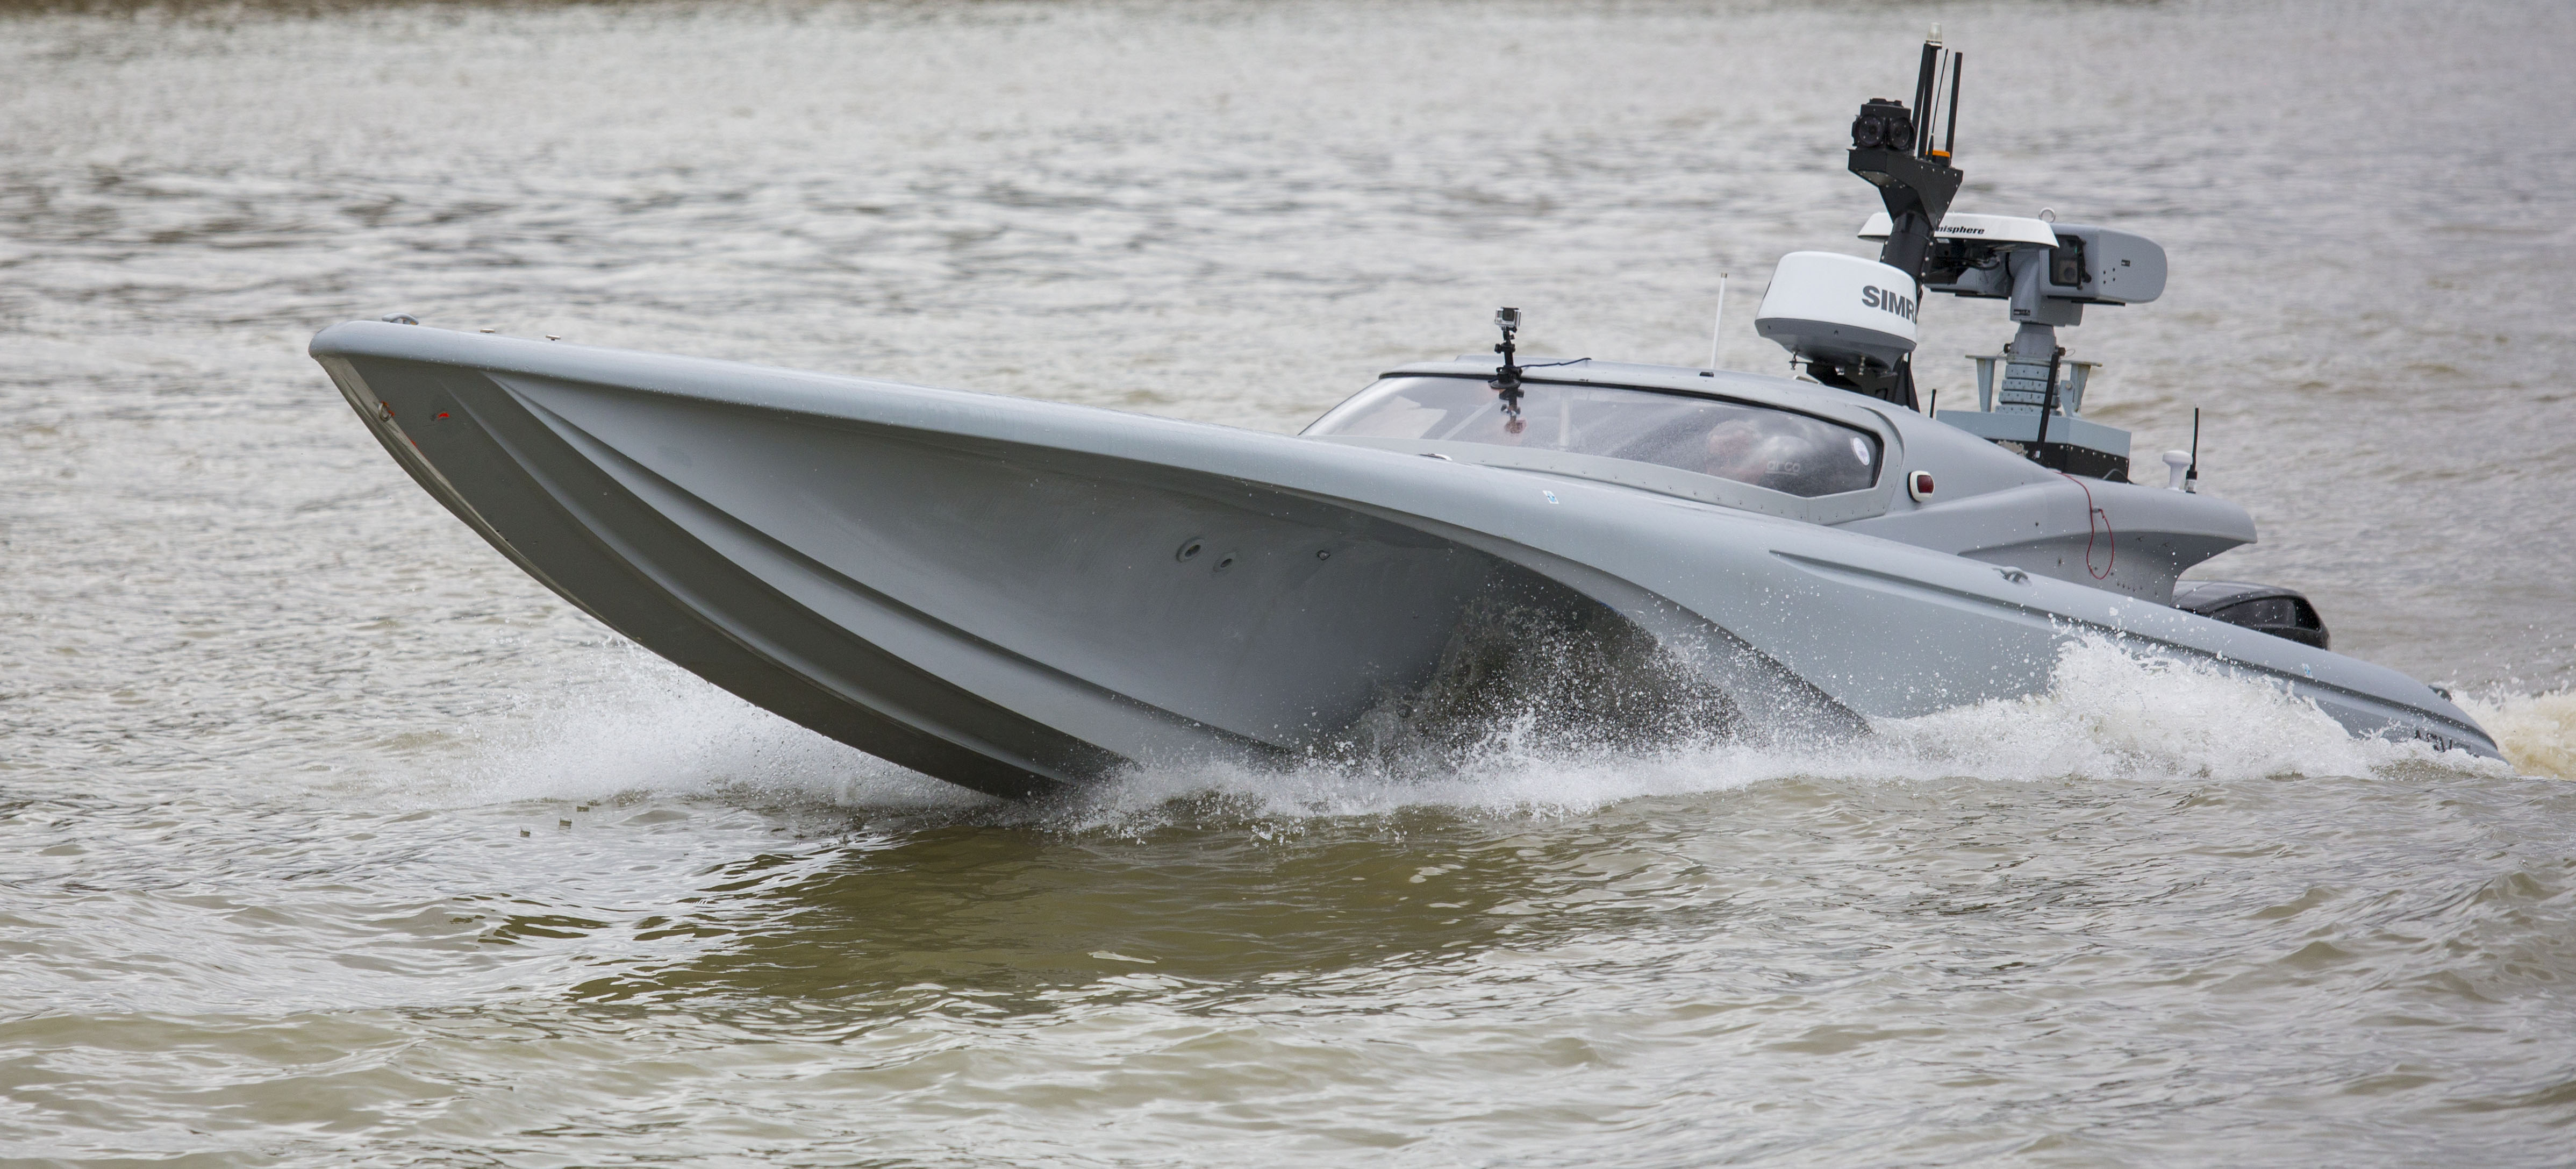
\includegraphics[width=\linewidth]{report/images/usv.jpg}
    \caption{Bladerunner craft fitted with the MAST (Maritime Autonomy Surface Testbed) system}
    \label{fig:my_label}
\end{figure}

\subsection{State}
\label{ss:state}
An agent's \textbf{state} is how it is represented and seen by other agent's in the environment. It contains the agent's current \emph{position} $(x, y)$ in metres, \emph{speed} $\agentspeed$ in m/s and \emph{heading} $\agentheading$ in radians.

where,
\hspace{0.5in}$x, y \in \mathbb{R}$
\hspace{0.5in}$\agentspeed \in \mathbb{R^+}$
\hspace{0.5in}$ \agentheading \in [0, 2\pi]$

\subsection{Constraints}
\label{ss:constraints}
Each agent is constrained by three kinematic constraints:
\begin{itemize}
    \item maximum speed $\maxagentspeed$
    \item maximum absolute change in speed $\maxdeltaspeed$ 
    \item maximum absolute change in heading $\maxdeltaheading$
\end{itemize}
Additionally, the speed of the agent is bounded below by 0 to avoid it trying to move in a reversed direction.
% $\agentcommand{a_i} : \mathbf{R^2} \rightarrow \mathbf{R^2}$, from a motion goal where \deltaspeed is the change in the agent's speed and \deltaheading is the change in the agent's heading.

\begin{figure}
    \centering
    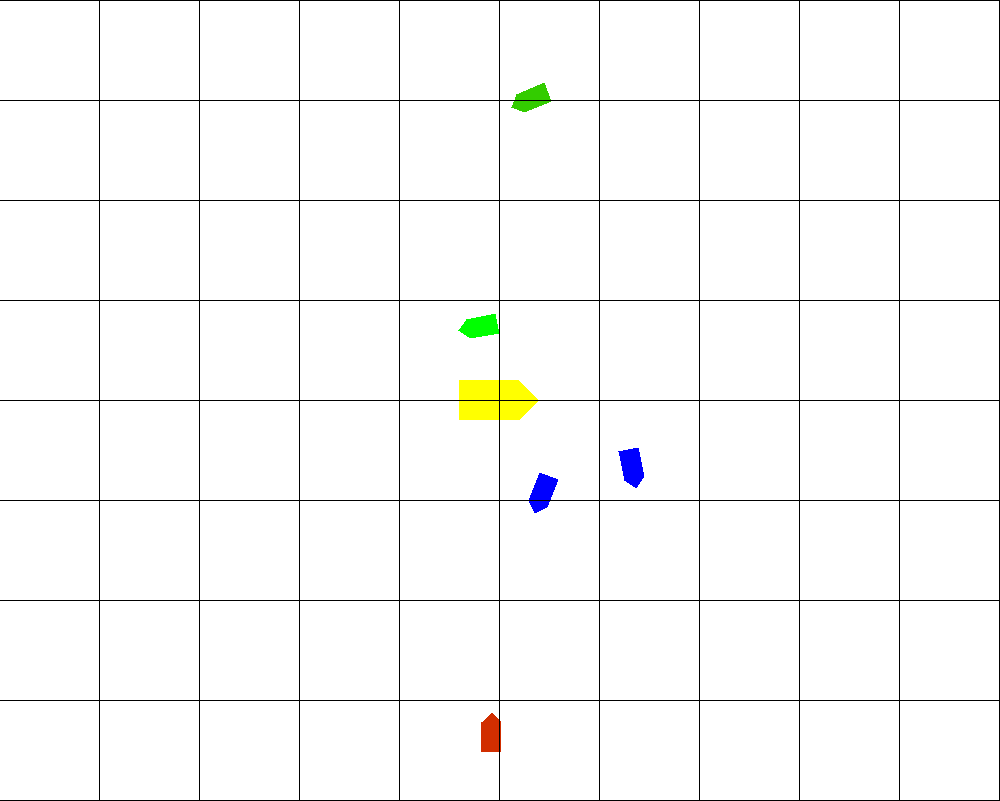
\includegraphics[width=0.8\linewidth]{report/images/agents.png}
    \caption{Figure displaying agent's interacting with each other in the simulation. Blue vessels are the USVs, Green vessels are intruders with low threat probability, and Red vessels are intruders with high threat probability}
    \label{fig:agents}
\end{figure}

\subsection{Collision Avoidance Parameters}
Each agent is equipped with a collision avoidance fan that has a parameterised radius and width. Furthermore, each agent has an aggression parameter $\aggression$. This parameter is responsible for how "aggressive" it is when avoiding obstacles. Further explanation is given in \ref{sec:control}.

\subsection{Motion Goals}
\label{def:mg}
A \textbf{motion goal} $\agentmotiongoal{\agent{i}} \in \mathbf{R}^2$ for an agent $\agent{i}$ is defined as the position to which an assigned agent will try to move towards. All agents, USVs, Intruders, and Assets have a motion goal assigned to them. However, these motion goals can depend on different things. For instance, if the intruder is a threat or \nonthreat or the task assigned to the USV. Furthermore, the assigned motion goal could also be a weighted combination of other assigned motion goals. 

\subsection{Commands}
\label{def:command}
A \textbf{command} is the action that an agent takes in reaction to the environment. For our purposes we assume that every agent can change their speed and heading through their commands. Hence, a command, $\agentcommand{a_i}=[\deltaspeed, \deltaheading]^T$ is a two dimensional vector containing the desired change in speed and change in heading for an agent $a_i$. 

\subsection{Task Assignment}
A \textbf{task} is assigned to USV's in order to request them to perform a particular. It's a structure containing a index and a type. The type refers to the behaviour~\ref{sec:behaviours} expected of the USV. The use of the index depends on the expected behaviour. For instance, in the case of the guard behaviour, the index refers to the guard position to take. However, in the case of delay and observe behaviours, the index refers to the target intruder. This is explained in more detail in section \ref{sec:behaviours}. A \textbf{task assignment}, $\taskallocation{} \subset \totaltaskset$, to USV $\usvagent{i}$  is a subset of the total set of tasks.

\section{Swarm Simulation}
This package contains the simulation and visualisation software used by the other sub-systems.

\subsection{Simulation}
The simulation software is responsible for the actual kinematics of the agents in the environment. For our purposes we discretise the timesteps of the environment and update the kinematics asynchronously with the other systems. I.e. kinematic update is done in its own process. This allows the simulation to not have to wait until it receives a command from the agent in order to update its kinematics. This is unlike openai's popular reinforcement learning environments which wait on a command/action before it can update the environment. This design allows for the following advantages: The agent's can interact concurrently in the environment, which is much more realistic. Agent's can work distributed without having to organise some sort of scheduling (e.g. Should we wait until all agents submit an action before updating and for how long?). 

This concurrency is possible because of the ROS subscriber and publisher architecture. Firstly, after performing the kinematic updates for each agent, the simulation publishes \texttt{WorldState} messages under the "Perception" topic. This  \texttt{WorldState} message is just a list of all the updated agents' state as described in \ref{ss:state}. It then subscribes to \texttt{AgentCommand} messages under the "Command" topic, which also follow the same structure as defined in \ref{ss:command}. When an agent receives a new command for an agent it is placed on a stack (of max size 1) in that agent's simulation object. Thus, when the simulation performs the kinematic update for that object, it pops the command of the stack, if there is one, and uses that for the update. The exact kinematic update is shown in the \texttt{Python} code below \ref{code:sim}.

\begin{lstlisting}[language=Python, caption=kinematic update for an agent in the simulation, label=code:sim]
def update_state(self, delta_t):
    self.lock.acquire()  # Acquire thread lock
    
    # Commands
    command = self.command
    delta_speed = command.delta_speed
    delta_heading = command.delta_heading

    # State
    pos_x = self.x
    pos_y = self.y
    speed = self.state[2]
    heading = self.state[3]

    # Update state
    heading += delta_heading*delta_t
    speed += delta_speed*delta_t
    pos_x += speed*np.cos(heading)*delta_t
    pos_y += speed*np.sin(heading)*delta_t

    # Set state
    self.x = pos_x
    self.y = pos_y
    self.speed = max(speed, 0)
    self.heading = heading
    self.lock.release() # Release thread lock
    self.command = None
    return self.state
\end{lstlisting}

\subsection{Visualisation}
Using \texttt{Python}'s \emph{tkinter} we were able to visualise results of our software stack, which was necessary for evaluation and debugging of the system. Figures \ref{fig:agents, fig:sim} are snapshots taking from the visualisation. In these figures you can see blue vessel shaped polygons which represent USVs. Green vessel shaped polygons which represent benign intruders. Red vessel shaped polygons which are intruders classified as malicious and a larger yellow vessel shape polygon representing the asset. The visualisation can also show useful debugging visualisation such as transitioning the colours of intruders from green to red as their probability of being a threat increases. Additionally, there are red circles indicating the motion goals of USVs and lines between USVs and Intruders which indicate that the USV has the intruder as either an Observed or Delay task.

The visualisation is also possible because of the ROS listener architecture. It listens to messages over the topics \emph{threatStatistics}, \emph{Markers} and \emph{Task\_Allocation} for debugging information. However, it gets the agent positions from the simulation directly because they're ran in the same process. 

\begin{figure}
    \centering
    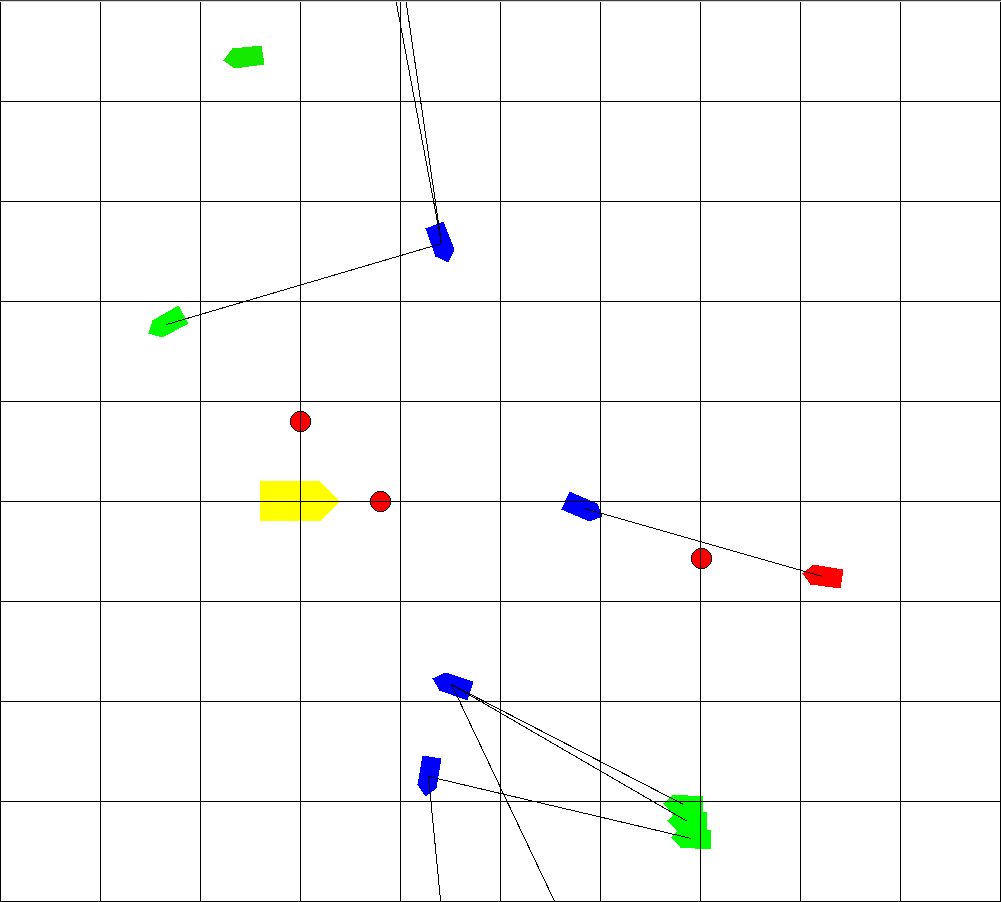
\includegraphics[width=0.8\linewidth]{report/images/sim.png}
    \caption{Snapshot of visualisation software.}
    \label{fig:sim}
\end{figure}

% \subsection{Implementation}
% The package \texttt{swarm\_core} is a core dependency for all packages in the system. It provides the system with necessary header files agent.h, swarm\_tools.h and ros\_swarm\_tools.h. 

% \subsubsection{agent.h}
% This file contains the definitions of the agents described above \ref{def:agent}. Also, it contains definitions for common structures used by the agents such as commands, tasks, constraints and collision avoidance parameters.

% \subsubsection{swarm\_tools.h}
% This file instead contains mathematical tools to be used by agents. 

% \subsubsection{ros\_swarm\_tools.h}
% This file contains definitions of functions responsible for extracting data from ROS msgs and converting it to the relevant structure for the agent to use. It is also responsible for doing the reverse operations.

\section{Swarm Control}
\label{sec:control}
\subsection{Collision Detection}
\label{ss:collision}
Collision detection is the process of determining whether two or more bodies are or will make contact with one or another in the foreseeable future \cite{4414258}.  This has applications from stationary single agent robotic manipulators \cite{galabally2018collision} \cite{6987848} to mobile multi-agent systems \cite{marzoughi2018collision}\cite{van2011reciprocal}. 
The collision detection system is based on the one proposed in \cite{raboin2013model}. Where it is assumed that each agent has a radar of a pre-specified radius and range. Furthermore, once an object, stationary or mobile, enters this region a collision is detected. 

\subsubsection{Collision Check}
Firstly, each object, stationary and mobile is given a radius (This is set to 50m for both intruders and USVs). Using this radius we can calculate the leftmost and rightmost edge points of this object from the perspective of an agent trying to avoid by using the algorithm \ref{}. If either the leftmost edge point or rightmost edge point falls within the range of the radar of the agent trying to avoid the object then a collision is detected.
%TODO Collision Check Algorithm


%\TODO reference algorithm
\begin{figure}
    \centering
    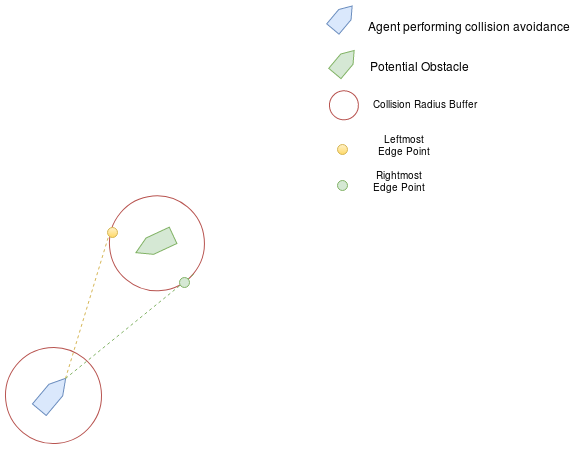
\includegraphics[width=0.8\linewidth]{report/images/edge_points.png}
    \caption{Edge points of potential obstacle}
    \label{fig:edge}
\end{figure}


\subsubsection{Occupied Intervals}
An occupied interval is an angle range indicating a range of headings 
 Edge points are then calculated for each vessel in the vicinity of the agent $\agent{i}$ performing collision avoidance. The collision check then marks $\agent{i}$ as a potential obstacle, then the angle of the edges in reference to $\agent{i}$ is calculated. 

\subsubsection{Safe Intervals}
The occupied intervals are firstly sorted from leftmost to rightmost. Then, iterating through the sorted occupied intervals we keep track of the rightmost edge. The idea being that if there is ever a gap between this rightmost edge and the next occupied interval, then the previously tracked rightmost point and the leftmost point of the occupied interval must be a safe interval and is then stored as such. Otherwise, if there is overlap with the rightmost point and the new occupied interval, then the tracked rightmost edge is then extended to the rightmost edge of the occupied interval.

\subsection{Collision Avoidance}
\textbf{Collision avoidance} is the act of adjusting an agent's current plan in order to avoid a detected collision. It is a staple in robotics and multi-agent systems \cite{marzoughi2018collision, 4414258, kuwata2011safe, galabally2018collision}. Additionally, when operating in the real world, all vessels are subjected to Convention on the International Regulations for Preventing Collisions at Sea (COLREG). These regulations dictate how your vessel takes evasive manoeuvres situations of potential collisions. Hence, if there's any future for USVs to operate in open water they must be able to follow these regulations. An example of this is seen in the work done by \citet{kuwata2011safe}, in which they focused on the USVs' reaction in three situations \ref{tab:colreg}. Figure \ref{fig:colreg} also illustrates the responses. For our collision avoidance system, we did not take into account COLREG stipulations. We chose not to do this due to time constraints. However, this is an interesting and necessary extension for further work.Instead the collision avoidance system used in this project works as a basic local planner. It receives a plan or in our case the desired command and adjust it to a command that is deemed safe by the system.

\begin{figure}
    \centering
    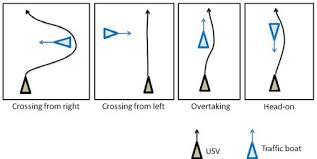
\includegraphics{report/images/colreg.jpg}
    \caption{Required manoeuvres for different COLREG situations \cite{kuwata2011safe}}
    \label{fig:colreg}
\end{figure}
\begin{table}[]
\begin{tabular}{|l|l|}
\hline
\thead{Situation}  & \thead{Required Response}                                                                                                               \\ \hline
\textbf{Crossing}   & The vessel that has the other on the starboard (right) side must give way.                                             \\ \hline
\textbf{Overtaking} & \makecell[l]{COLREGs does not specify which side to overtake, but it is common practice \\ to overtake on the right.}                         \\ \hline
\textbf{Head-on}    & \makecell[l]{Both vessels must alter their course on starboard (right), so that they pass\\ with the other vessel on their port (left) side.}\\ \hline
\end{tabular}
\caption{Description of COLREG required responses in different potential collision situations}
\label{tab:colreg}
\end{table}

\subsubsection{Adjusting Change in Speed Command $(\deltaspeed)$}
\label{sss:colspeed}
The system implemented only adjusts the desired $\deltaspeed$ if the collision detection fan is completely blocked. At that point of complete obfuscation, the system attempts to reduce the speed to zero, bringing the vessel to a complete stop. \citet{raboin2013model} suggests to use the largest interval, however, this produces undesirable behaviour with the agent taking large deviations from the desired command even though a smaller deviation was feasible. Using the nearest safe angle interval $(\theta_{l}, \theta_{r})$, $\deltaheading$ is assigned as the following:

\begin{algorithm}
\caption{$\deltaspeed$ weighted assignment}
\begin{algorithmic}
\IF{$|\theta_{l}-\deltaspeed|<|\theta_{r}-\deltaspeed|$}
\STATE $\deltaheading \leftarrow \aggression\theta_{l} + (1-\aggression)\theta_{r}$
\ELSE
\STATE $\deltaheading \leftarrow (1-\aggression)\theta_{l} + \aggression\theta_{r}$
\ENDIF
\end{algorithmic}
\end{algorithm}

\subsubsection{Adjusting Change in Heading Command $(\deltaheading)$}
\label{sss:colheading}
When adjusting  $\deltaheading$ the system considers three cases:
\begin{enumerate}
    \item The desired change in heading is not deemed unsafe by the collision detection system. 
    
    \hspace{24pt}--- No change to the desired command
    
    \item There entire collision avoidance fan is blocked so no action is deemed safe 
    
    \hspace{24pt}--- It adjusts the speed as explained in \ref{sss:colspeed}

    \item The desired command was deemed unsafe 
    
    \hspace{24pt}--- Adjusts heading until it is deemed as safe.
\end{enumerate}
	
From here on we will focus on the third case described above. As mentioned above, the collision avoidance system will return a list of safe intervals. Using the list of returned safe intervals the collision avoidance system calculates the nearest safe interval to the current $\deltaheading$ desired command. 

\begin{figure}
    \centering
    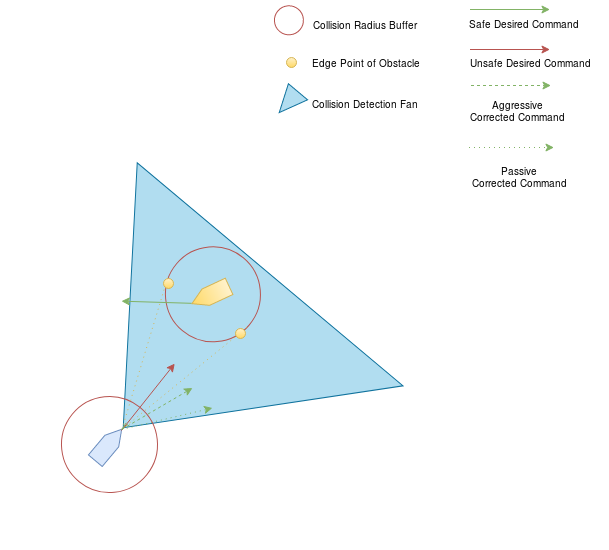
\includegraphics[width=0.8\linewidth]{report/images/corrected_command.png}
    \caption{Demonstration of collision avoidance system detecting and avoiding obstacle}
    \label{fig:ca}
\end{figure}

\subsection{Behaviours}
\label{sec:behaviours}
In this section the Behaviour's used by the USV's will be described in detail.
\subsubsection{Observe Behaviour}
\label{ss:beh:observe}
When a USV is undertaking the observed Behaviour it gets a motion goal on the line between the intruding vessel and the asset $\agentlocation{observe} = \agentlocation{intruder} + \w_{observe}(\agentlocation{asset}-\agentlocation{intruder})$ formula. where this point is located on the line is determined by a weight w which depends on the threat probability of the intruding vessel and the distance between the intruding vessel and the asset. It should be noted that once the threat probability of a vessel exceeds a prespecified threshold the observed Behaviour becomes a delay Behaviour. More on this in %link section [task allocation section]
$$w_{observe} = \gamma_{obs}\threatprob{j}(1+\frac{\gamma_{dist}}{|\agentlocation{intruder}-\agentlocation{asset}|})$$
%TODO Insert Weight Formula 

\subsubsection{Guard Behaviour}
\label{ss:beh:guard}
This Behaviour produces a motion goal on a circle with a fixed radius surrounding the asset. These motion goals are equally spread around the fixed asset. Hence,
$$\agentmotiongoal{guard} = \left[r_{guard}cos(\tau), r_{guard}sin(\tau)\right]^T \bigoplus \agentlocation{asset}$$
% TODO possibly expand more

\subsubsection{Delay Behaviour}
\label{ss:beh:delay}
The delay Behaviour produces a motion goal on the line between the intruding vessel and the asset $\agentmotiongoal{delay} = \agentlocation{intruder} + \alpha_{delay}(\agentlocation{asset}-\agentlocation{intruder})$ much like the observe Behaviour. However, the weight w for this Behaviour is a bit more complicated than the observe Behaviour weight. 

The is the problem of finding $\alpha_{delay}$ such that,
    $$\agentmotiongoal{delay} = \agentlocation{intruder} + \alpha_{delay}(\agentlocation{asset}-\agentlocation{intruder})$$
subject to,
    $$\frac{|\agentlocation{}-\agentlocation{usv}|}{\agentspeed_{usv}} = \frac{|\agentlocation{}-\agentlocation{intruder}|}{\agentspeed_{intruder}}$$

This actually simplifies to a quadratic equation in $\alpha_{delay}$ 

    $$A\alpha_{delay}^2 + B\alpha_{delay} + C=0$$

where,
\begin{align*}
    0 &< \alpha_{delay} < 1 \\
    A &= |\boldsymbol{o}|^2(1-(\frac{\agentspeed_{usv}}{\agentspeed_{intruder}})^2)\\
    B &= 2\boldsymbol{d}\cdot(\boldsymbol{o})\\
    C &= |\boldsymbol{d}|^2\\
    \boldsymbol{o} &= \agentlocation{intruder}-\agentlocation{asset}\\
    \boldsymbol{d} &= \agentlocation{usv}-\agentlocation{intruder}
\end{align*}

% \begin{figure}
%     \centering
%     % \includegraphics[scale=0.5]{report/images/behav.png}
%     \caption{Figure showing motion models of different behaviours \cite{raboin2013model}}
%     \label{fig:my_label}
% \end{figure}

\subsection{Intruder Behaviour}
\label{sub:beh:intruder}

If an intruder is malicious then its motion goal is the location of the asset. 

More formally,

$$\agentmotiongoal{\threatintruder_j} = \agentlocation{asset}$$

$\text{For every \threat intruder \hspace{}} \threatintruder_j \in \threatintruderset$

When the intruder is not a threat then it follows the behaviour learned behaviour model described by the intruder model in section \ref{}. This is a strong deviation from what \citep{raboin2013model} initially presented. The original \nonthreat intruders defined in \cite{raboin2013model} would would move from their randomly initialised point, to a randomly assigned motion goal on the other side of the asset. Additionally, they would move along a circle centred around the asset with randomly initialised radius. The intruder model we proposed is learnt from real-world vessel traffic data. Details of this model can be found in \ref{}.

\subsubsection{Control Command}
The goal for each agent is to get to its motion goal in the fastest and safest way possible. Specifically, every agent tries to travel at its maximum speed, except in the case when their obstacle fan is completely blocked \ref{sss:colspeed}. Additionally, the agent will try to make the smallest change in heading, except again in the case when collision avoidance takes over \ref{sss:colheading}. However, if an intruder is in the act of evading, it will purposefully take the larger change in heading.

\subsubsection{Control Pipeline}
Every agent in the environment has the same control pipeline:
\begin{itemize}
    \item Calculate new motion goal given its state, the state of the other agents and their current task allocation (Again in the case of USVs).
    \item Use this motion goal to get a desired command.
    \item Run the desired command through the collision detection system. If a collision is detected then the collision avoidance system will take over.
    \item Publish \texttt{AgentCommand} message under /Commands topic.
\end{itemize}

\section{Swarm Task Allocation}
Task allocation in a multi-robot system is the problem of determining which robots should execute which tasks in order to achieve the overall system goals \citep{korsah2013comprehensive}. Thus, the task allocation package is responsible for finding the best allocation of tasks, $\usvtaskallocation{j} \subset \taskallocation{d} \cup \taskallocation{g} \cup \taskallocation{o}$, for each usv agent in our team of usv's $\usvset$ to do to maximise the delay of malicious intruders $\threatintruderset \subset \intruderset$. 

The task allocator runs in a separate process to the USVs, and at each allocation refresh step, the swarm task allocation package sends a request to the model-predictive simulation service~\ref{def:service} advertised by each USV. Each USV has this service and is responsible for performing a local search based around the current task allocation and returning the best result. They perform this search by first generating the candidate swarm assignments following the algorithm given in \ref{ss:generate}, forward simulating how the agents will interact in the environment and evaluating the results of the simulation using the heuristics mentioned in \ref{ss:heuristics}. The agents then find the best assignment out of the candidates, by using a heuristic on the predictions and submitting that assignment along with it's weight from the heuristic as the response. The task allocator, then chooses the best assignment out of the submitted assignments and allocates that as the new assignment. In the following sections I describe the algorithm used for generating candidate swarm allocations to be evaluated during the local search, the model predictive simulation algorithm that forward predicts how the agents will interact in the environment given they are assigned the candidate swarm allocation and finally the heuristics used during evaluating the result of the model-predictive simulation. 

\subsection{Generating Candidate Swarm Assignments}
\label{ss:generate}
When deciding on the next best swarm assignment, a local search is performed around the current swarm assignment. During this local search candidate swarm assignments are generated and are then evaluated. Candidates are constructed by performing either an exchange~\ref{sss:exchange} or a share~\ref{sss:share}. The process by which the candidates are generated is described below and the full algorithm can be found in appendix \ref{alg:gen} Exchange operations take place when the tasks are the same type. If they are, then their indexes are exchanged, else nothing happens. If the two indexes are equal then the index of the other usv is set to -1 indicating that this task is to be dropped. Share operations takes place if the main usv has a delay task and the other usv does not. When this happens, the delay task is added to the other usv.

\subsection{Model-Predictive Simulation}
\label{ss:mpsimulation}
For each candidate swarm allocation, the current world state is sampled. Where sampling the world state, samples the intruder classification as a threat or non-threat based on their threat probability. Then for each sample the world is forward predicted in discrete timesteps. Every timestep, each of the agents follow their control pipeline. For intruders classified as threats, we assume their motion goal is the asset's position. Originally, we wanted to query the benign intruder model inside the task allocation loop. But, this caused the task allocation update to slow down drastically. However, through analysis of the ais dataset, we confirmed our hypothesis that vessels for the most part don't take drastic manoeuvres. Thus, during the model-predictive simulation period, we assume that the benign vessels do not change their current trajectory (except when collision avoidance takes over). This is repeated until the max timestep is reached or an intruder has reached within a predefined threshold of the asset.

\subsection{Heuristics}
\label{ss:heuristics}
\inlinecomment{TODO}

\chapter{Experiment Setup}
\chapter{Experiment Results}
\chapter{Conclusion}
\appendix

% use the following and \cite{} as above if you use BibTeX
% otherwise generate bibtem entries
% \bibliographystyle{plain}
\bibliography{mybibfile}

\end{document}
